\chapter{Introduction}
\addcontentsline{toc}{chapter}{Introduction}
\chaptermark{Introduction}
\label{sec:background}
A fundamental grasp of the data that is produced by sequencing biological organisms is essential to comprehend the research outlined in this manuscript. If already familiar with DNA sequences, how they are obtained and how they differ between species or individuals, you may proceed to section~\ref{sec:background:pangenomics} \emph{From reads to \kmers}.
\section{DNA, genome variation and sequencing data}
\label{sec:dna}
DNA (Deoxyribonucleic Acid) is a complex molecule with a double helix structure that carries the genetic information of an organism. Although its discovery was the result of work by many scientists over nearly 90 years, the currently accepted model was first correctly described by James Watson and Francis Crick in 1953 at Cambridge, UK.\\
The information DNA carries provides instructions for an organism to develop, survive in the external world, and reproduce. These instructions are encoded as a sequence of monomers called nucleotides. Each nucleotide is composed of a sugar, a phosphate group, and one of four nucleobases: cytosine, guanine, adenine, and thymine. The nucleotides are commonly referred to using the first letter of their nucleobases: A, C, G, and T. In RNA molecules, thymine is replaced by uracil.\\
The nucleotides are linked together in a sugar-phosphate backbone. Hydrogen bonds between complementary nucleotides form the molecule's double-stranded structure, with A pairing with T and C pairing with G bases. This pairing is crucial for DNA replication and protein synthesis. Figure~\ref{fig:DNA} shows the structure of the DNA molecule and the nucleotides, with the initial drawing by Francis Crick in 1953.
\begin{figure}[h!]
	\centering
	\begin{subfigure}[b]{0.95\textwidth}
		\centering
		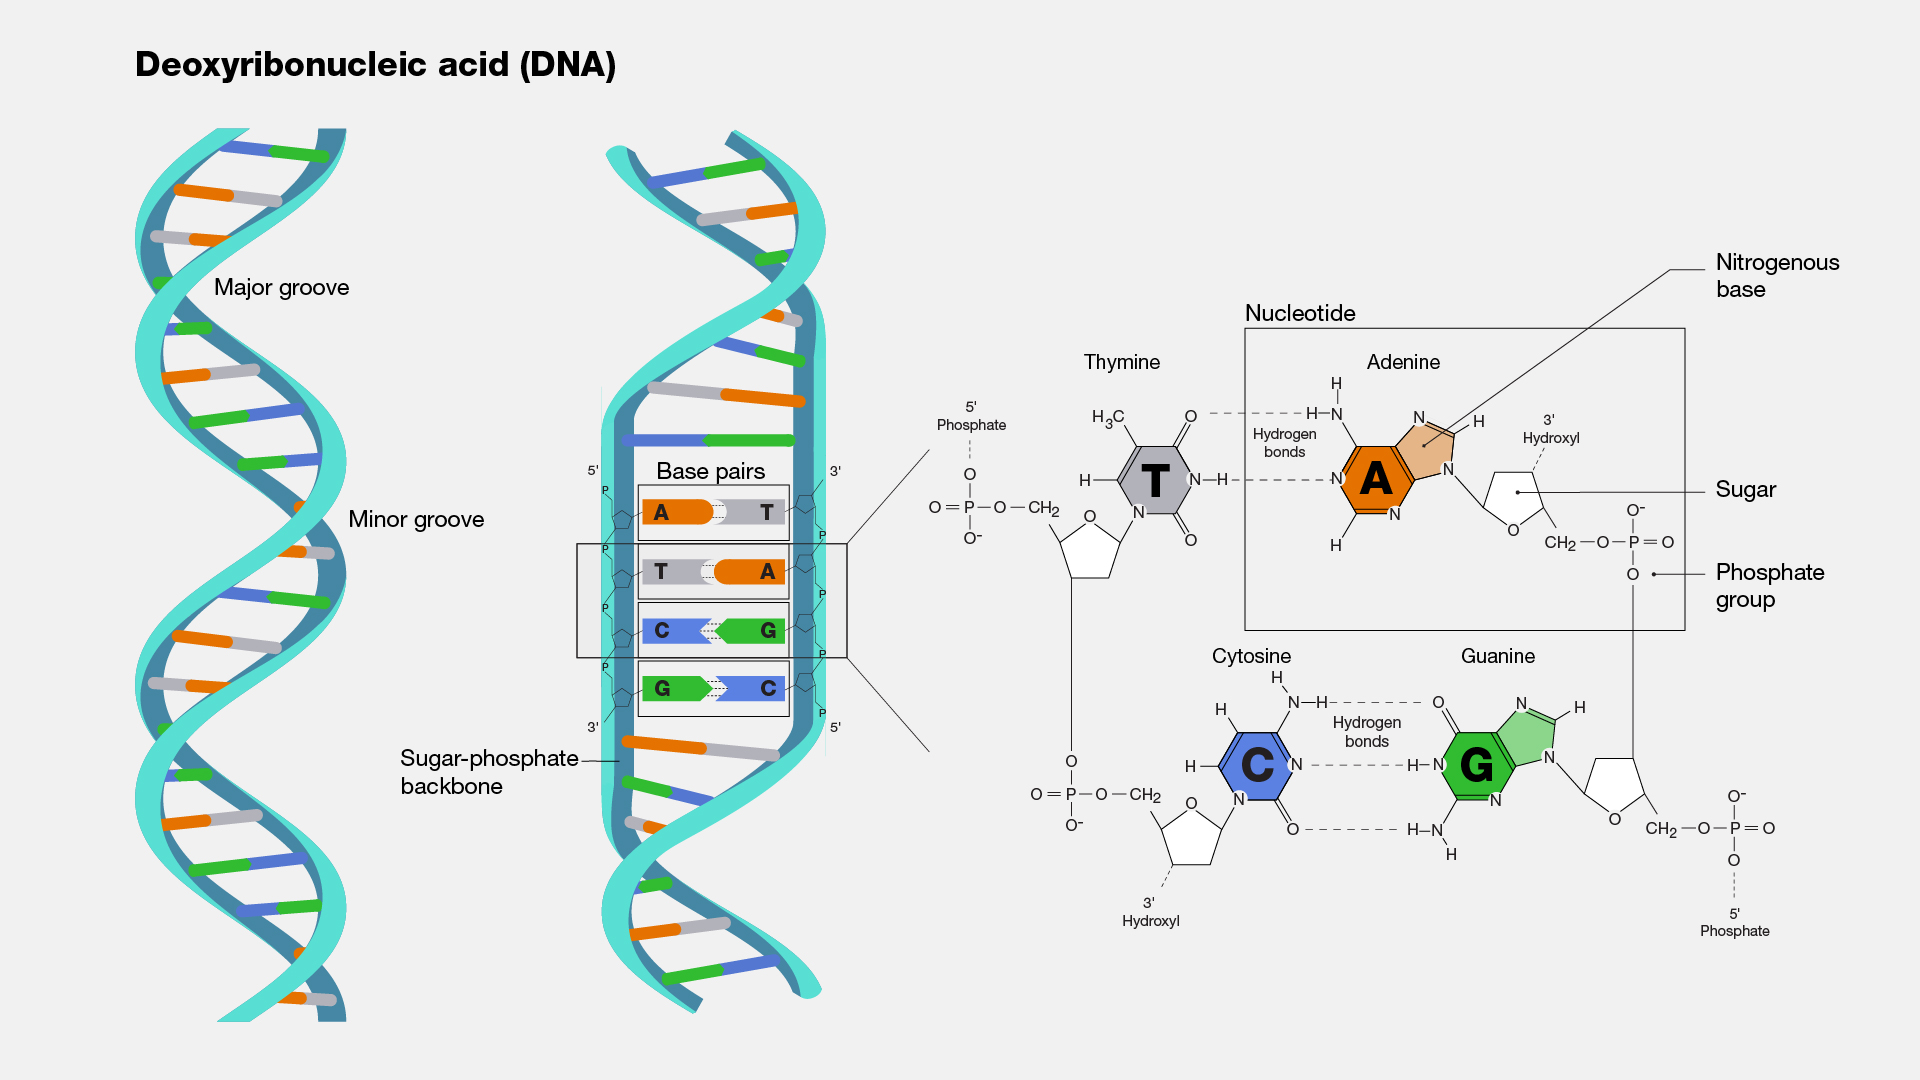
\includegraphics[width=0.95\textwidth]{figures/background/DNA_2024a.jpg}
		\caption[The DNA molecule]{The DNA molecule and the structure of the nucleotides, the basic piece of information of the DNA. Figure from NIH glossary~\cite{nih_dna}.} 
	\end{subfigure}%
	\\
	\begin{subfigure}[b]{0.75\textwidth}
		\centering
		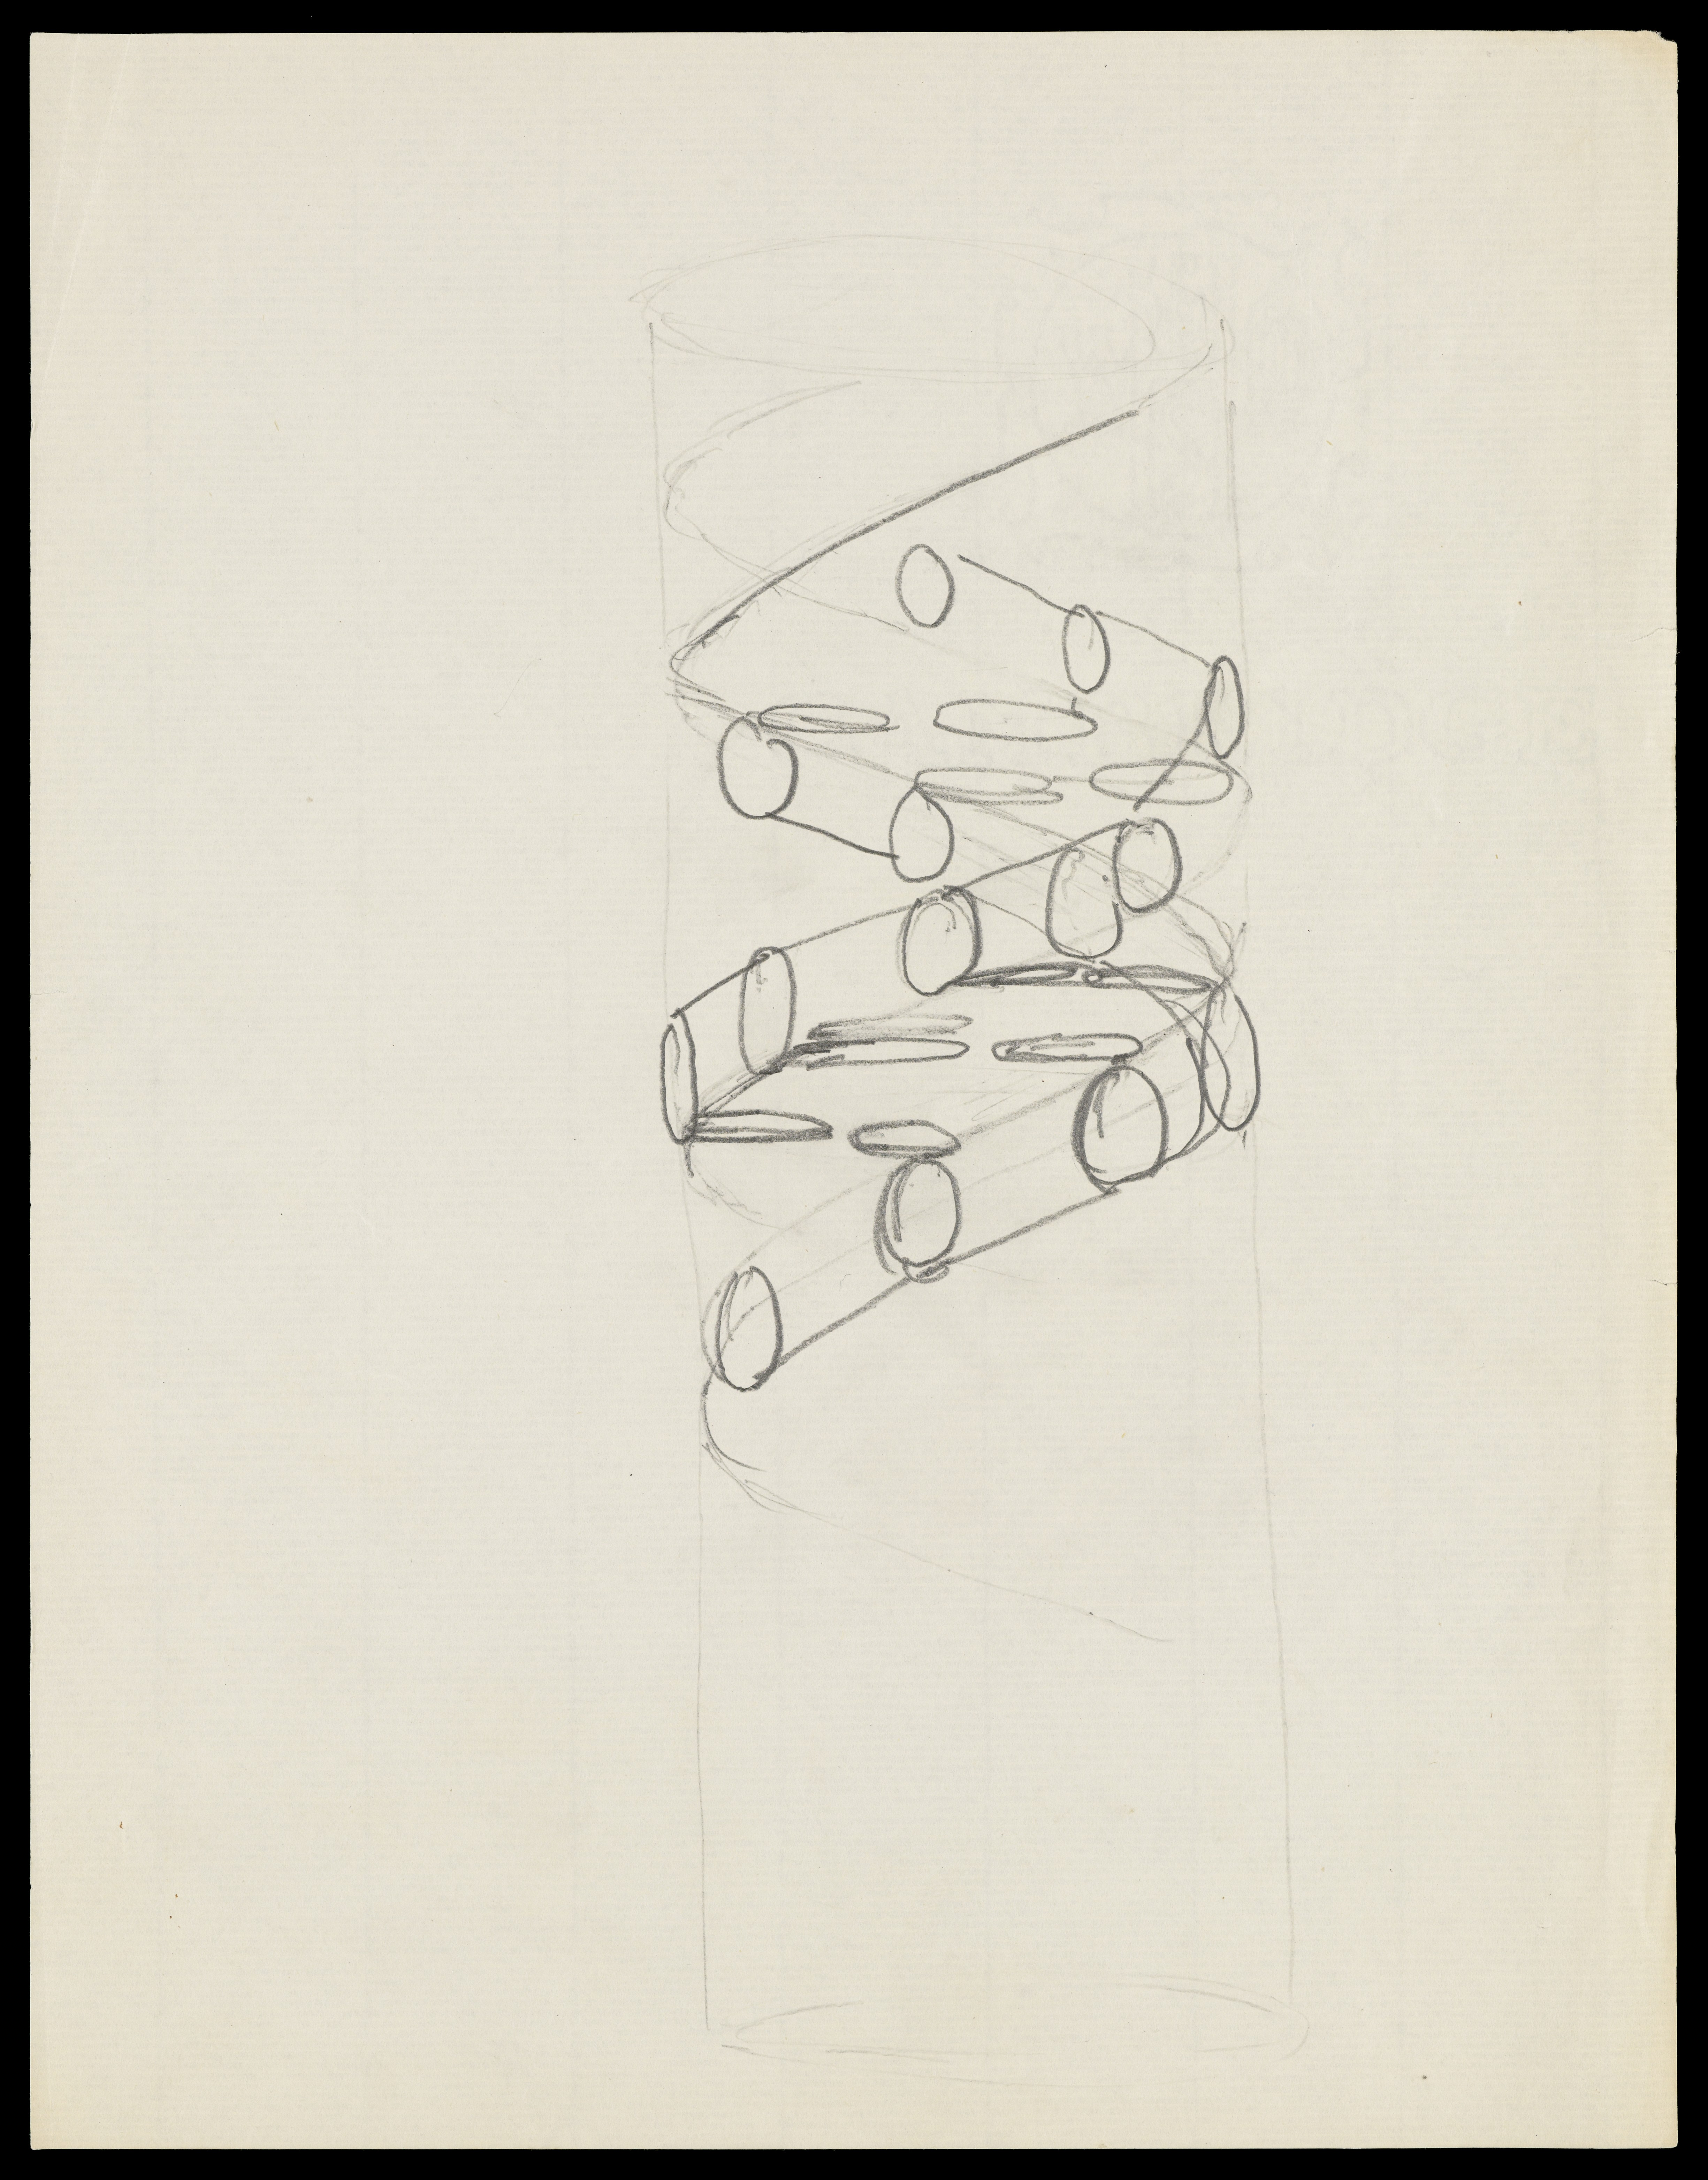
\includegraphics[width=0.5\textwidth]{figures/background/DNA_sketch.jpg}
		\caption[The DNA sketch by Crick]{The DNA molecule model draw by Francis Crick in 1953.} 
	\end{subfigure}%
\caption{The DNA molecule.}
\label{fig:DNA}
\end{figure}

To fit inside the cell nucleus, DNA is organized in very tight structures. First is coiled around proteins called histones to from a compact structure called chromatin that form loops and is kept in place by other molecules to structure a chromosome. Chromosomes are inherited by the offspring through sexual or asexual reproduction. Humans are diploids, i.e. contain 2 copies of the same chromosome, that receive one copy from the mother (the egg) and one from the father (the sperm). Both the egg and the sperm (the gametes) contain 1 copy of the chromosomes. While mammals are often diploids, other organism can be haploid (one single copy of the chromosome) or polyploid, i.e. have more than 2 copies. For example, the sugar cane plant, the world's most harvested crop by tonnage, can have more than 8 copies of a chromosome, up to 12~\cite{sugarcane}.
In humans, each nucleus of non-reproductive cells contains 23 chromosome pairs. 22 are the autosomes, i.e. the chromosomes we all have and that are not associated with sex, while the last pair is the sex one that contains or 2 copies of chromosome X for women or 1 X and 1 Y for men. The final part of the chromosome is called telomere while the central one is called centromere and both are regions known to contain a lot of repetitive regions that are very difficult to reconstruct from sequencing. \\ Finally, there is also the mitochondrial genome, that is not in the nucleus, has circular structure and is mostly inherited maternally.

\subsection{DNA sequencing}
In many biological disciplines, studying an organism's genetic information contained in its DNA is crucial. Over the years, researchers have developed various methods and techniques to extract this information from the cell nucleus: these take collectively the name of genome sequencing. Sequencing can be thought as the way we observe genomes, i.e. by sequencing fragments of DNA and assembling them computationally\cite{garrison_pangenome}. 
These processes typically involve three main steps. Here I describe them, with many simplifications, to give a brief overview:
\begin{itemize}[leftmargin=1.8cm]
	\item[\textbf{Library preparation}] The first step requires hours long, nontrivial biological manipulation of samples to extract DNA from cell nucleus and purify it without causing damage. This process isolates the genetic material from other cellular components, like RNA and proteins. The DNA molecule are fragmented into pieces of different length followed by $5\prime$ and $3\prime$ adapter ligation. Some technologies require PCR amplification of fragments, while others don't.
	\item[\textbf{Sequencing}] Next, specialized machines detect the sequence of nucleotides that compose the extracted DNA pieces. These techniques, called sequencing, use various, most of the time proprietary, technologies to determine the precise order of nucleotides (A, C, G, and T) in a DNA molecule. The raw data output of these machines are sequences of characters that are referred to as sequencing reads or simply reads.
	\item[\textbf{Analysis}] In this step usually quality control (QC) is performed to remove adapters and too short or low quality reads. Usually the first step after QC is to assemble the sequences together or to provide them as input to a workflow specific for the required application.
\end{itemize}
The landscape of DNA sequencing has evolved significantly since its inception. In 1977, Frederick Sanger and his colleagues introduced the first widely adopted sequencing method, known as chain termination sequencing or Sanger sequencing\cite{sanger_sequencing}. This technique allowed to read the sequence of nucleotides in a DNA molecule for the first time in a reliable and reproducible manner. This was the technique that led to the first sequencing of the mitochondrial DNA and the first ,almost, complete human genome in 2001~\cite{mitochondrialDNA,first_human_genome}. Sanger technology through a gel produced the first reference genomes for important organisms.
While Sanger sequencing has revolutionized genetic research, it has largely been replaced by more advanced technologies. These newer methods fall into two main categories: Next Generation Sequencing (NGS) and Third Generation Sequencing. These technologies provide significant improvements in terms of speed, cost-effectiveness and data output compared to Sanger sequencing. \\
\subsubsection{Next Generation Sequencing} (NGS) derives its name by launching a so-called next generation by revolutionizing sequencing with massive parallelization. This technology has continuously improved since 2005 to yield up to 8 Terabases per single sequencing run, taking it maximum 2 days and dropping the price of, for example, a single individual sequenced per almost 100 dollars~\cite{100dollars}. The advancement consists mainly in running many reactions and analysis in parallel to produce millions to billions of reads of a length that varies between 150 and 300 bases. For this reason they take the name of short reads. While a big advantage of this sequencing method is the low error rates, with at least 80\% of the bases with less than 1 error in 1000 (i.e. 99.9\% accuracy). This technology is mostly dominated by a California biotechnology company called Illumina \\
The sequence length is the main drawback of this method. As they are too short to assemble into a high-quality \emph{de-novo} complete genome, they are used for \emph{re-sequencing}, i.e. to be mapped to a reference genome to infer variations from it, to be used, for example, in population variation studies. Additionally, the short length of the fragment makes sequences coming from parts of the genome not in a reference or from complex and/or repetitive regions often impossible to be mapped, loosing all the information associated to them.
%won't align to any part of a reference genome to be used to infer from which part of a chromosome it comes from. The same problem arise for repetitive regions,like centromeres, telomeres or small segmental duplications, that have a length greater than the sequence length, where it is not possible to asses the length or the nature of the repetition. 
This problem has been partially addressed by the introduction of pair-end sequences, a technology that is now integrated in all Next Generation machines, that sequences both ends of a single DNA fragment and then associate the two reads that come from it, in order to provide more long-range information. Although this method is still not enough to solve complex variations, it is very useful to track some of the reads that would be instead be discarded and finds relevant applications in other fields, like metagenomics. In fact, I used this property of paired-end reads in one method I developed before the PhD to improve the estimation of different species inside environmental samples sequenced with NGS~\cite{metaprob2}. \\
Finally, this technology enabled also other kind of sequencing, like STARR-seq, ATAC-seq, ChIP-seq, RNA-seq and others, that enabled to assay regulatory activity in the genome.
\subsubsection{Third Generation Sequencing} (TGS) is the newest technology that uses alternative approaches to NGS, to solve the issues that it currently face due to the short length of the sequences. The main difference relies on the fact that while NGS uses PCR to amplify the small fragments in which DNA is broken into prior to sequencing, these new technologies directly sequence the nucleic acids in their native form. For this reason they are called single molecule technologies.\\
Here I will describe the two most important technologies, provided by the two companies that lead this market: a California biotech company called Pacific Biosciences, usually called PacBio, and a Uk based one, called Oxford Nanopore Technologies, or ONT.\\
PacBio offers "HiFi sequencing" that produces reads long up to 25 thousands bases in length with accuracy comparable to NGS ones. This is achieved by first creating a circularized DNA from high-quality double stranded DNA and then using a DNA polymerase enzyme to read multiple times the same molecule to produce a final consensus sequence with accuracy of around 99.9\%. These are long and accurate reads that enable ultra-fast assembly of human genomes~\cite{mdbg} at a cost around \$1000 per sequencing reagents kit for a 30X coverage of a human genome. \\
Oxford Nanopore machines instead provide ultra-long sequences, that are on average longer than the PacBio HiFi ones and can reach up to the megabase scale (i.e. ~100 times longer). The sequencing is done by passing a single-strand DNA molecule trough a tiny nanopore. Each pore is associated to an electrode and a sensor that measure the current that is passing through the pore. As the DNA goes through the pore, the current changes and, thanks to a basecalling algorithm, it is possible to detect the nucleotides by the change in the current. This process is done in parallel across ~800-1500 pores.\\
It is finally important to stress that these two technologies allow the detection of all kind of variations, i.e. small variations as well as large ones and also solve large repetitive regions as they span across thousands of bases. Moreover, both these methods allow the direct detection of DNA methylation. This is a chemical mechanism on top of the DNA molecule that regulates gene expression  by recruiting proteins involved in gene repression or by inhibiting the binding of transcription factor(s) to DNA~\cite{methylation}. \\
Figure~\ref{fig:sequencing_technologies} shows basic schematics of how these two technologies work.\\ 
\begin{figure}[h!]
	\centering
	\begin{subfigure}[b]{0.95\textwidth}
		\centering
		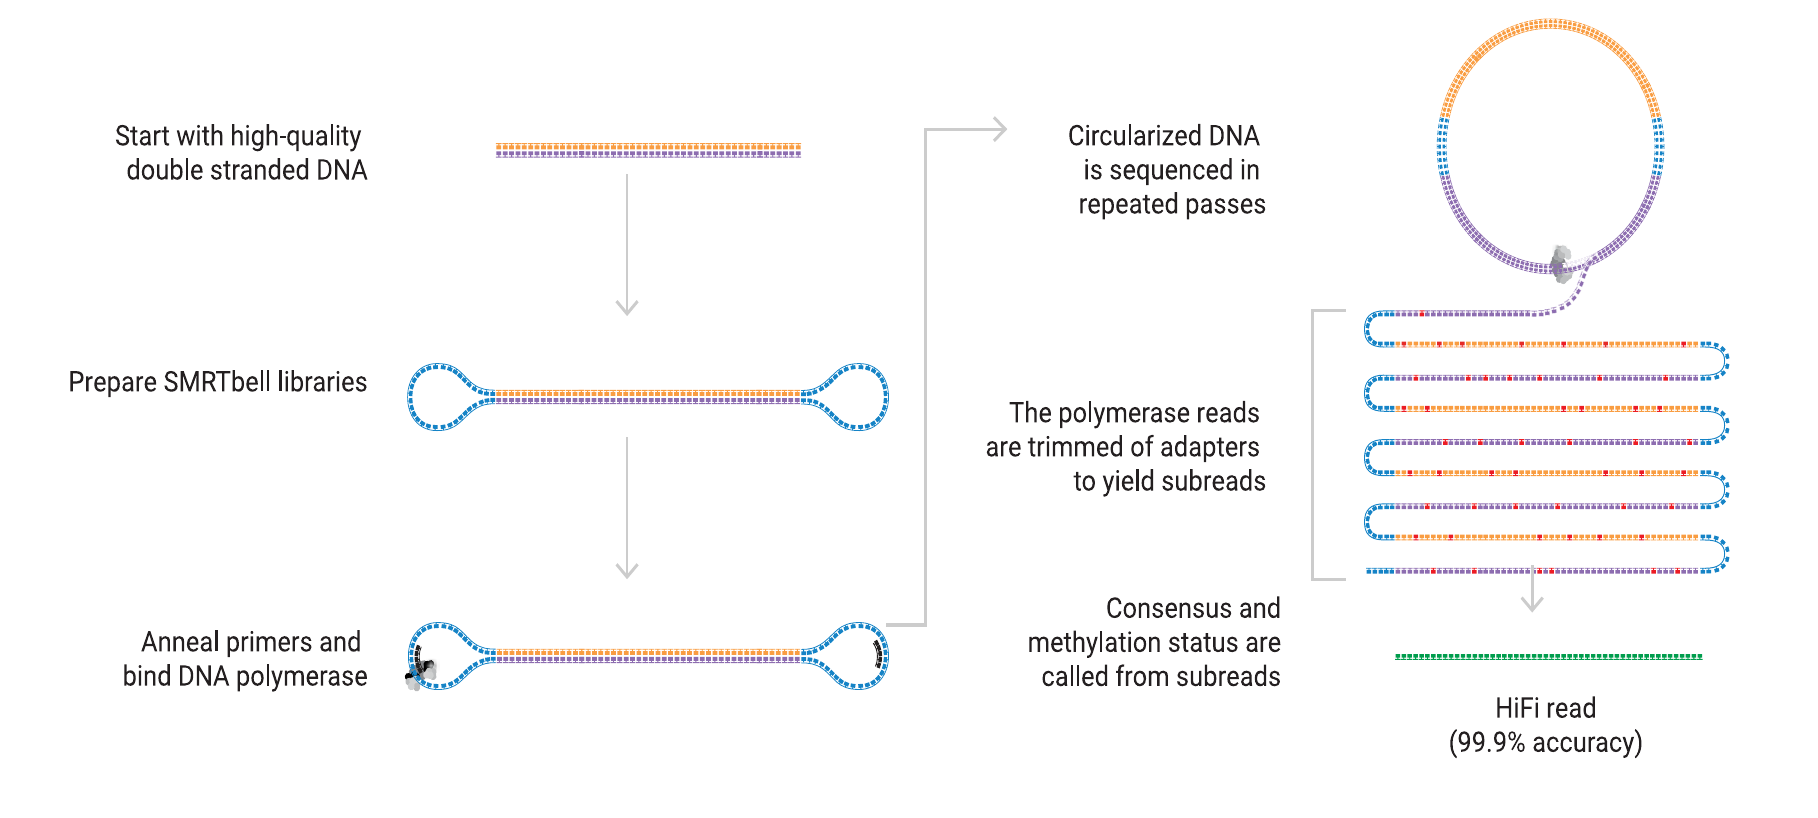
\includegraphics[width=0.95\textwidth]{figures/background/hifi_pacbio.png}
		\caption{Pacific Biosciences Hi-Fi reads generations scheme. Image from PacBio website.} 
	\end{subfigure}%
	\\
	\begin{subfigure}[b]{0.95\textwidth}
		\centering
		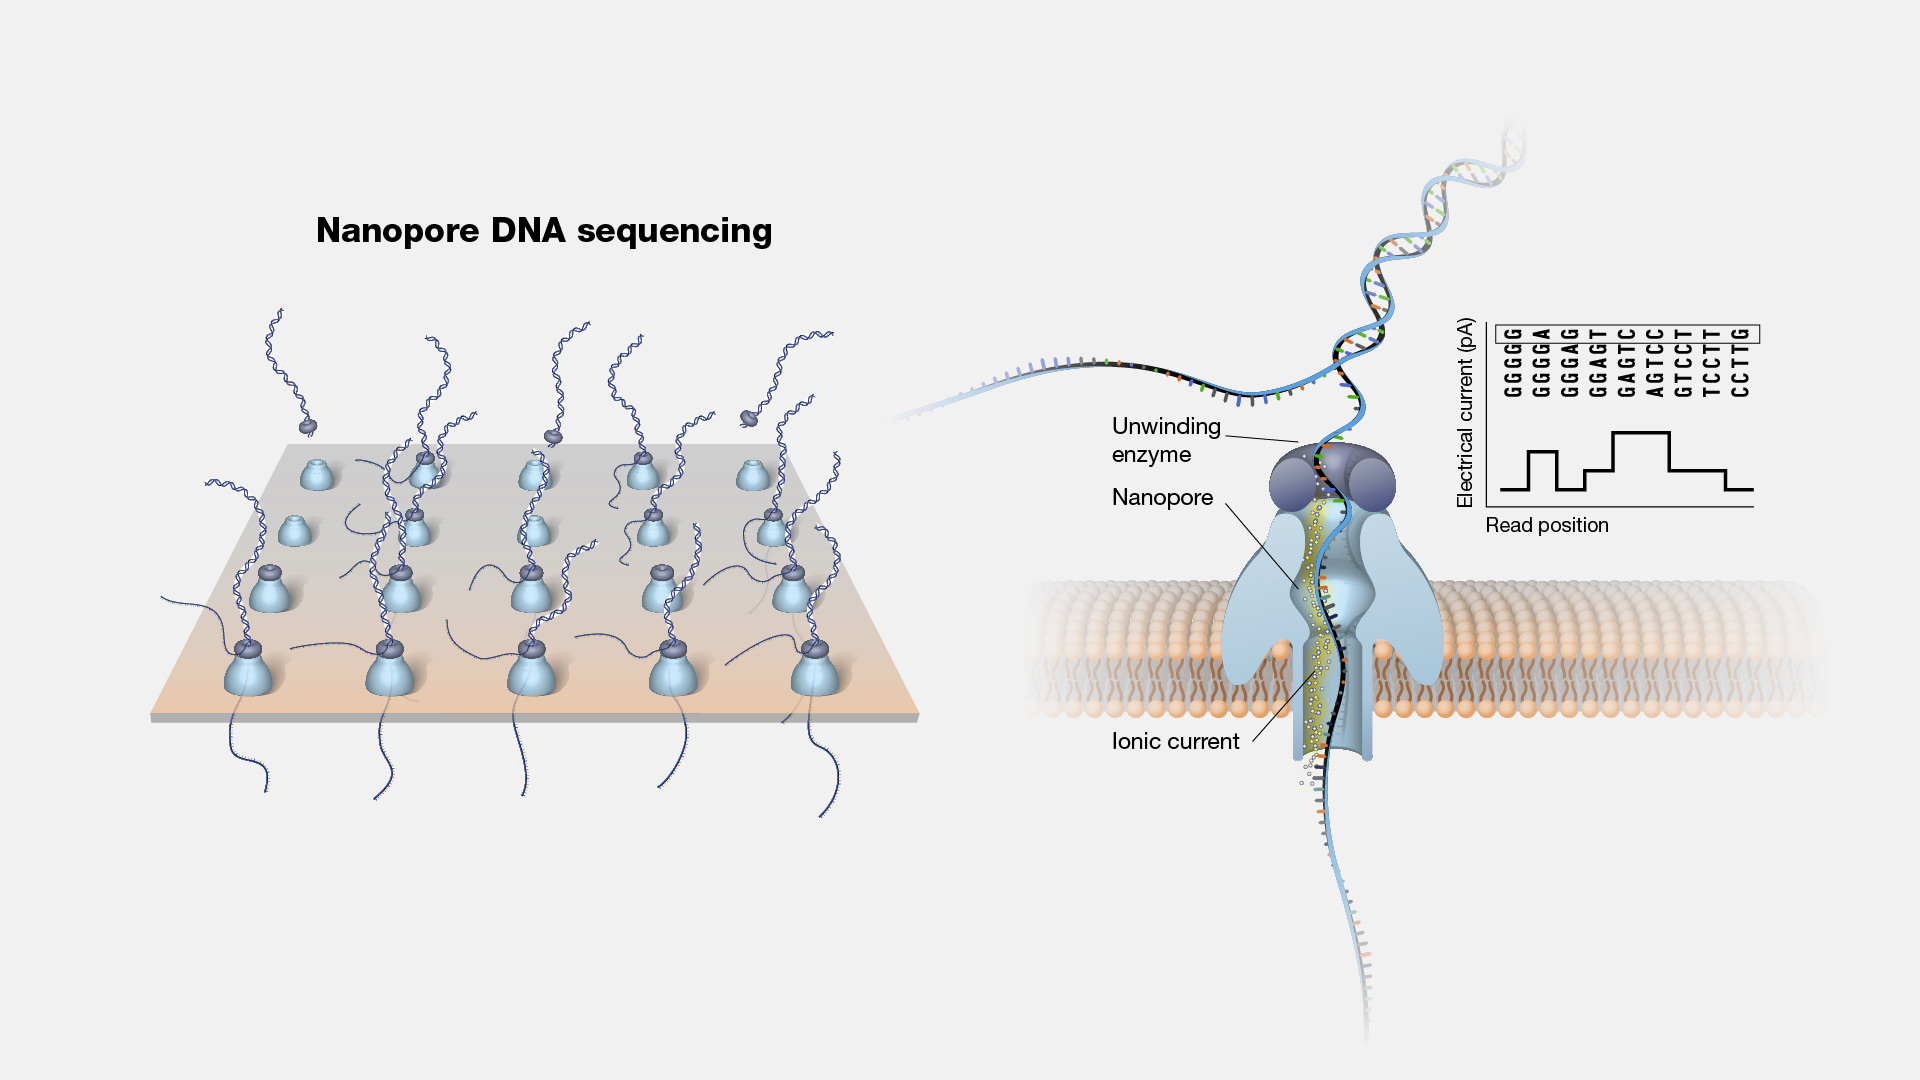
\includegraphics[width=0.95\textwidth]{figures/background/nanopore_sequencing.jpg}
		\caption{An array of pores sequences multiple molecules in parallel. A dsDNA molecule is split by the helicase enzyme and then a ssDNA sequence slowly gets through the pore for sequencing. Changes in the ionic current is used by a machine learning algorithm to infer the nucleotides of the sequence.} 
	\end{subfigure}%
	\caption{Third generation sequencing technologies.}
	\label{fig:sequencing_technologies}
\end{figure}

\section{From reads to \kmers}
The sequences produced by any of the aforementioned technologies are considered as text strings, i.e. successions of characters, like the phrases of this manuscript, in which each character correspond to a nucleotide. These sequences can therefore being stored in plain text formats, like FASTQ, that preserve basecalling quality information or in others, like FASTA, that retains only the actual sequence. In order to use less space and take advantage of redundancy in the sequencing data, these files are often compressed, using one of the many tools publicly available like \texttt{gzip} or \texttt{zstd}, by Facebook. \\
As pair-end short-reads have different features than ultra-long reads or Hi-Fi long reads, most of the tools focus on providing applications for just one single type. In cases like assembling a genome from the reads or calling the variant of the sequenced genome compared to one of reference, however, the information from different sources can be combined to provide superior results. In order to generate high-quality genome assemblies, for example, many consortia, like the Human Pangenome Reference Consortium, use Hi-Fi long reads as bases for assembly plus ultra-long reads as scaffolds to chain together the assemblies into sequences that span from telomere to telomere of a chromosome.\\
In the work presented in this manuscript, most of the tools will ingest as input or raw sequences (both NGS or TGS) or high-quality, near telomere-to-telomere assemblies. Some of the tools that I have have used and all of the ones I have developed or co-developed transform the input sequences or assemblies into \kmers to produce the desired output. \\
\begin{description}
	\item[DNA alphabet] The DNA alphabet $\sum$ is composed by the 4 characters that compose the first letter of the nucleobases: A,C, G and T: $ \sum = {A, C, G, T}$, 
	\item[sequence] a biological sequence from $\sum$ is defined as $ S =\in \sum^{l}$, with $\lvert S \rvert = l $, with length $l$ that can be fixed, if originated from NGS, or variable, if originated from TGS.
	\item[\kmer] a \kmer of $S$ is defined as $ \kmer \in \sum^{k}$, with $\lvert \kmer \rvert = k $ i.e. any valid sub-string of $S$ of length $k$. 
\end{description}
As shown in table~\ref{tab-kmers}, from any sequence $S$, it is possible to obtain its constituent \kmers. To efficiently extract all \kmers from a sequence, the best approach is to employ a sliding window technique. This is done by identifying the first \kmer at the start of the string and then iteratively shifting the window one position at a time, appending the newly encountered character to the right while removing the leftmost character.\\ The length $k$ of a \kmer is an arbitrary value, that is usually chosen depending on the kind of sequences used (cannot have $k$ > $n$), the characteristics of the data that is used (is it from a single organism, a collection of the same species, a collection of different organisms) and on the disk or memory space that is available for computation or storage (as in table~\ref{tab-kmers}, the longer the $k$, the more space is used by repetitive characters). A more detailed explanation of these considerations will be provided in section XXX[QF].\\
As it is possible to retrieve \kmers from a single read, it is trivial to extend this property to any set of reads, for example produced by a single sequencing run of a sample. This means that a set of \kmers is equivalent to the set of reads it is obtained from. In order to characterize this transformation as lossless, i.e. without any loss of information, an association from each \kmer to the read(s) it comes from would be needed. In most of the cases this is not useful and \kmers are obtained from reads without remembering from which reads do they come from. In other, specific, applications it might instead be needed to know in which reads there are certain \kmers. More considerations on this are going to be presented in section XXX[BackToSequences].\\
As presented in section~\ref{sec:dna} the DNA is double-stranded, with A bases are paired with T ones, while C bases are paired with G ones, also called complements. If a \kmer appears in a sequence, in the other strand of the molecule there would be what is called its reverse complement. This is the spelling of the \kmer from the end to the beginning, substituting each base with its complement. For example if in one strand there appear the sequence $ACGT$, on the other strand it would spell $TGCA$.\\
When enumerating \kmers from a sequence or when storing them, only "canonical" \kmers are kept: this means that for each \kmer produced from a sequence, its reverse-complement is computed and only the one that is considered smaller by a certain property is kept. For example, if the lexicographic order is used, the \kmer (with $k=4$) $ACGT$ is lexicographically smaller than $TGCA$ so when either of the two is seen, only the first is kept.\\
A classic operation that is done when enumerating \kmers from sequences is to keep track of how many times each canonical \kmer appears in the set of sequences. This is called \kmer counting and finds important applications in many genomic disciplines like metagenomics or transcriptomics.\\
\kmers are being used in lots of applications based on NGS short reads while they are less implied on methods for error-prone long reads because using \kmers on one side destroys the long range information provided by reads that span thousands of bases, on the other error-rates higher than NGS would produce too many erroneous \kmers that would be very difficult to correct if not with very deep sequencing, providing additional cost bottlenecks. With Hi-FI reads and improved quality of nanopore basecalling, it is possible to overcome the error limitation and use \kmers for long reads. One example that uses advanced concepts based on \kmers is the tool \mdbg that drastically improved assembly of Hi-Fi reads.\\ 
\begin{table}[h!]
\begin{center}

	\begin{tabular}{ c c c c c c c c c c c}
		\toprule
		Position & 1 & 2 & 3 & 4 & 5 & 6 & 7 & 8 & 9 & 10 \\
		\midrule
		Sequece $S$ & C & T & G & A & A & C & T &A & C & A\\
		\midrule 
		$3-mers$ & C & T & G  \\
		&   & T & G & A \\
		&   &  & G & A & A \\
		&   &  &  & A & A & C\\
		&   &  &  &  & A & C & T\\
		&   &  &  &  &  & C & T & A \\
		&   &  &  &  &  &  & T & A & C \\
		&   &  &  &  &  & & & A & C & A\\
		
		\hline
	\end{tabular}

	\vspace*{0.3 cm}

	\centering
	\begin{tabular}{ c c c c c c c c c c c}
	\toprule
	Position & 1 & 2 & 3 & 4 & 5 & 6 & 7 & 8 & 9 & 10 \\
	\midrule
	Sequece $S$ & C & T & G & A & A & C & T &A & C & A\\
	\midrule 
	$4-mers$ & C & T & G & A \\
	&   & T & G & A & A\\
	&   &  & G & A & A & C\\
	&   &  &  & A & A & C & T\\
	&   &  &  &  & A & C & T & A\\
	&   &  &  &  &  & C & T & A & C\\
	&   &  &  &  &  &  & T & A & C & A\\

	
	\bottomrule
\end{tabular}
	\caption[\kmer computation from a sequence]{\kmers with $k=(3,4)$ being computed from the sequence \texttt{S} = \texttt{CTGAACTACA}. $l-k +1$ $k$-mers are generated for a total of $(l -k + 1) * k$ bases. While with $k=3$ the total bases are $ 8 * 3 = 24$, with $k=4$ they are instead $28$, as larger $k$ encodes more information redundancy.}
	\label{tab-kmers}
\end{center}
\end{table}


\begin{table}
\begin{center}
	\begin{tabular}{c | c}

		Sequence id & sequence \\
		\hline
		seq1 & ACATCA \\
		seq2 & CTTCAG \\
		seq3 & TACAGC \\
		seq4 & GCTTAC \\
		
	\end{tabular}
\newline
\vspace*{0.2 cm}
\newline

	\begin{tabular}{c | c | c | c  | c}

		Sequence id & seq1 & seq2 & seq3 & seq4\\
		\hline
		\kmers  & \underline{ACA} (TGT) & CTT (\underline{AAG}) & TAC (\underline{GTA}) & GCT (\underline{AGC}) \\
			    & CAT (\underline{ATG}) & TTC (\underline{GAA}) & \underline{ACA} (TGT) & CTT (\underline{AAG}) \\
				& \underline{ATC} (GAT) & \underline{TCA} (TGA) & \underline{CAG} (CTG) & TTA (\underline{TAA}) \\
				& TCA (\underline{TGA}) & \underline{CAG} (CTG) & \underline{AGC} (GCT) & TAC (\underline{GTA}) \\
	\end{tabular}
\newline
\vspace*{0.2 cm}
\newline

	\begin{tabular}{c | c}

		oredered caonical \kmer & count\\
		\hline
		AAG & 2 \\
		ACA & 2 \\
		AGC & 2 \\
		ATG & 1 \\
		ATC & 1 \\
		CAG & 2 \\
		GAA & 1 \\
		GTA & 2 \\
		TAA & 1 \\
		TCA & 2 \\
	\end{tabular}
\end{center}
	\caption[Example of canonical \kmer counting.]{Example of canonical \kmers enumeration and count. Given a set of sequences, for each of them \kmers are computed in a stream. For each of them, on the fly, the reverse complement is computed. Then the ones that are considered canonicals are passed and counted.\\ In the table below, reverse complements are between parenthesis and the canonical between the two (by lexicographic order) is underlined.}
	\label{tab-lista-kmer}
\end{table}

\clearpage

\section{Genetic diversity: focus on humans.}
\label{sec:background:pangenomics}
%Genomic variations are the characteristics that produce differences between organism of a species or between species. 
The Human genome contains more than 3 billions base pairs and contains probably more than 20 thousands protein coding genes, i.e. specific parts of the DNA that serve as blueprint for proteins. The rest is non-coding, i.e. is not a gene but can serve as regulatory element, like enhancers, promoters and silencers or as other conserved, functional element. Differences in specific regions cause phenotypic changes that can increase, decrease or not affect the fitness of an individual.\\
Genetic diversity is the variability that exists between organisms at the genetic level, i.e. differences in the information enclosed in their DNA. It is the raw material for biological evolution as, without heritable genetic differences between us, we would not be able to biologically evolve. Here what I will present is valid for humans, as the large part of my work has been with human DNA sequences. Most genetic changes have no effect at all on the individuals carrying them but some can result in phenotypic differences.\\
\subsection{Causes and drivers of genetic diversity in humans}
There are two main mechanisms of genetic diversity: the arise of new mutations and the reshuffling of already present genetic material trough recombinations and duplications. Mutations are produced by physical or chemical damage, for example caused by UV radiation, prior cell division or by errors in the DNA replications during cell division. When this occurs in germinal cells they are transmitted to the offspring, while when happening in a somatic cell (not reproductive), the mutation is not transmitted but can instead be responsible for certain type of cancer. In humans, it is estimated that a newborn carries on average 70 point mutations (one nucleotide substitute with another), 15 from the mother and 55 from the father. The amount of mutations is proportional with the age of the person and, more than induced by replication, it is due to not corrected damage.\\
On top of the mutations, chunks of chromosomes from the mother and the father chromosomes are shuffled to produce new combinations. The effect of this random process produces the differences between siblings with the same biological parents. Recombination is heterogeneous in the DNA and depends on some motifs that promote higher recombination. Finally, recombination is also influenced by the age, mostly of the mother, as older mothers tend to produce offspring with more misplaced recombinations, also causing the well known trisomy 21.\\
Without diverging too deep into population genetics, it is also important to understand how new variations are conserved, lost or fixed (become prevalent) in a population. These outcomes are driven by two main factors: genetic drift and natural selection.\\
Genetic drift is a process, given by the randomness in the individuals that reproduce in a specific population. This can contribute to the loss or fixation of some variants just because of randomness and not because they provide an advantage to the individual. Specifically, in populations with small number of reproductive individuals, this can fixate detrimental variants, while in large populations, the large number of individuals buffers the event. \\
Natural selection, on the other hand, is a mechanism that explains human evolution: as genetic variations causes the gain or loss of specific phenotypic traits, these traits can confer positive or negative advantage compared to the rest of the individual in a population (fitness). This phenomenon can contribute selecting certain variations in a population by either contribute to the fixation or the loss of a variant. This mechanism explains our species adaptation to nutritional resources, climate and pathogens: in 10 thousand years a mutation in a gene that conferred the ability to digest milk has almost got fixed in humans, selection on certain genes explains better adaptations to cold or high altitudes and selection in HbS or DARC alleles has helped humans adapt and survive malaria infections\cite{genome_diversity_quintana}. 
\subsection{Human Genomic variation: types of variants}
There are various types of genomic variants: from the shortest, the single-nucleotide variants (SNV) or Single Nucleotide Polymorphism (SNP) when it is present in at least 1\% of the population, is the difference of one nucleobase between two individuals. In a specific part of the genome one person can have instead of a cytosine (C) a thymine (T), like for the SNP located 14 thousands bases upstream of the lactase gene that enables the lactase persistence mentioned earlier\cite{lactase_persistance}.
A second group of small variants is made of insertions and deletions (called together \emph{indels}): these are events in which it is present or missing a group of less than 50 nucleotides. The number of nucleotides is an arbitrary threshold used to better separate them from other kind of variations. Specific types of indels are the tandem repeats that, as the names suggests, are insertions or deletions of small repeated sequences of DNA. These repetitions usually are one after the other with no other sequence in between~\cite{nih_variation}.\\
\begin{figure}[h!]
	\centering
	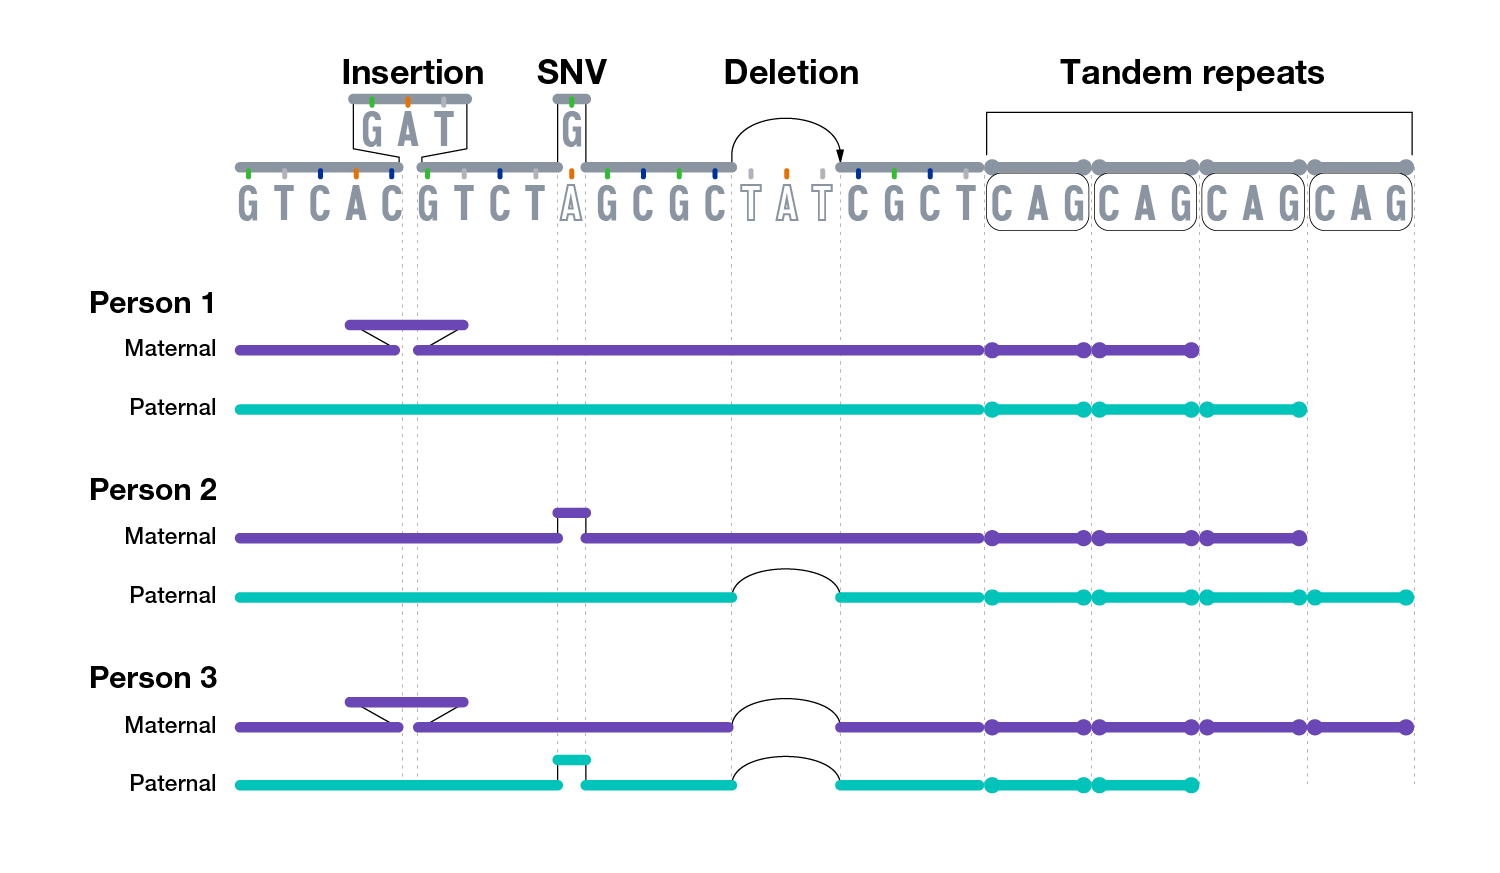
\includegraphics[width=\linewidth]{figures/background/small_variants.png}
	\caption[Small genomic variants.]{Graphic showing the types of small genomic variants~\cite{nih_variation}}
	\label{fig:small_variants}
\end{figure}
These groups of small variants, shown in figure\ref{fig:small_variants} are the most described, studied and associated with diseases as they were the only one consistently detectable with NGS sequencing. For these reason, studies that tried to associate genomic variation with diseases commonly used only these kind of variants.\\
The other kind of variations are the ones that stretch at least 50 nucleobases and that can reach the dimension of large chunks of the chromosomes: they are called structural variations (SVs).
These can be indels or tandem repeats with the repeated section longer than 50 nucleotides, accounting for nearly half of all SVs, that take the name of Copy Number Variants (CNVs). Moreover, there are also inversions, in which a chunk of DNA is inverted compared to another and translocations in which pieces of two different chromosomes trade places~\cite{nih_variation}.\\
\begin{figure}[h!]
	\centering
	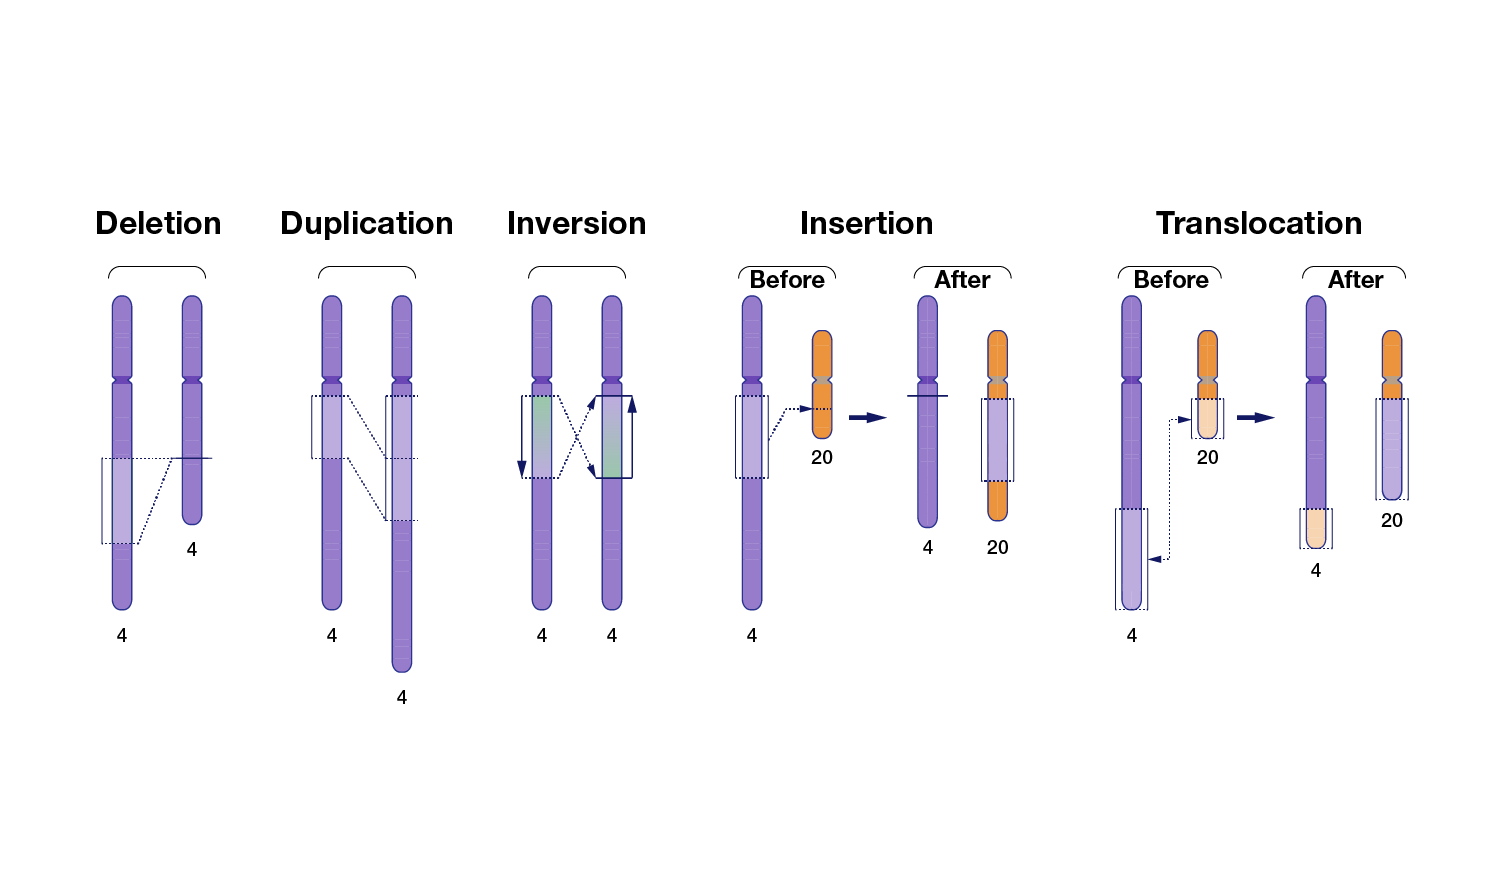
\includegraphics[width=\linewidth]{figures/background/large_variants.png}
	\caption[Large genomic variants.]{Graphic showing the types of large genomic variants~\cite{nih_variation}}
	\label{fig:large_variants}
\end{figure}
Finally, it is important to remember that these kind of variations can be on just one haplotype (copy of the chromosome) or on both: this distinguish between heterozygous and homozygous alleles.


\subsection{The importance of studying genomic diversity in populations context}
DNA differs between individuals of the same population (inter-individual) and between different populations of the same species (inter-population): figure~\ref{fig:pop_diff} shows the percentage of inter-individual variation for four close primates. Different species can differ in the amount of genetic variation that is s As discussed before, differences in DNA are given by having a different nucleotide at the same place (SNV), indels and large and complex variations, up to Megabases, that can produce different counts of copies or different ordering of a same region. \\
On average, each human carries around 10 thousands amino-acid altering mutations, 300-400 gene disruption events (like stop, splice and indels) affecting 200-300 genes and is heterozygous at 50-100 mutations associated with an inherited disorder~\cite{genome_diversity_quintana}. 
Finally, even when close species share a large portion of genetic material, structural changes that rearrange the same material in different order or invert it, contribute to meaningful changes. In figure~\ref{fig:chromosome_diff} it is shown how the chromosome 7 and 16 of some primates, even if very similar, differs in terms of organization. These large structure rearrangements are thus fundamental to understand the biology of organisms.
It is 
This is because the variation in DNA is produced by two main mechanisms: mutations and recombination. 

Moreover, genetic diversity is driven by two main factors: genetic drift and natural selection. Genomic duplication followed by adaptive mutation is considered one of the primary forces for evolution of new functions.
\begin{figure}[h!]
	\centering
	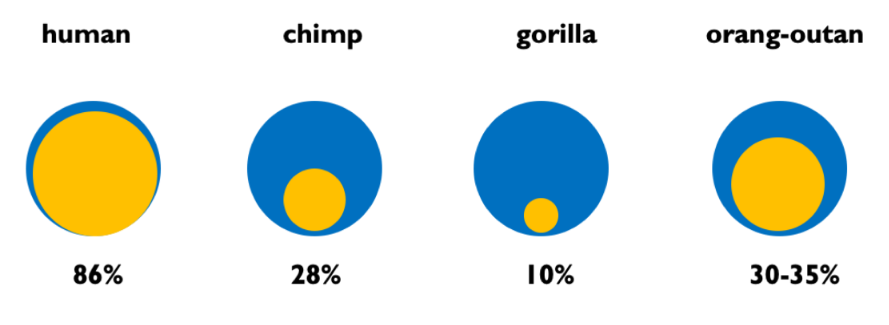
\includegraphics[width=.8\linewidth]{figures/background/pop_diff.png}
	\caption[Inter-individual and inter-population variation for 4 primate species.]{Share of inter-individual (yellow) and inter-population (blue) diversity for four different primates. While for humans the  majority of the diversity is within populations, for other primates it is between populations. This shows how Humans are more mixed than other primates. Percentage shows the inter-individual variation share~\cite{genome_diversity_quintana}.}
	\label{fig:pop_diff}
\end{figure}

\begin{figure}[h!]
	\centering
	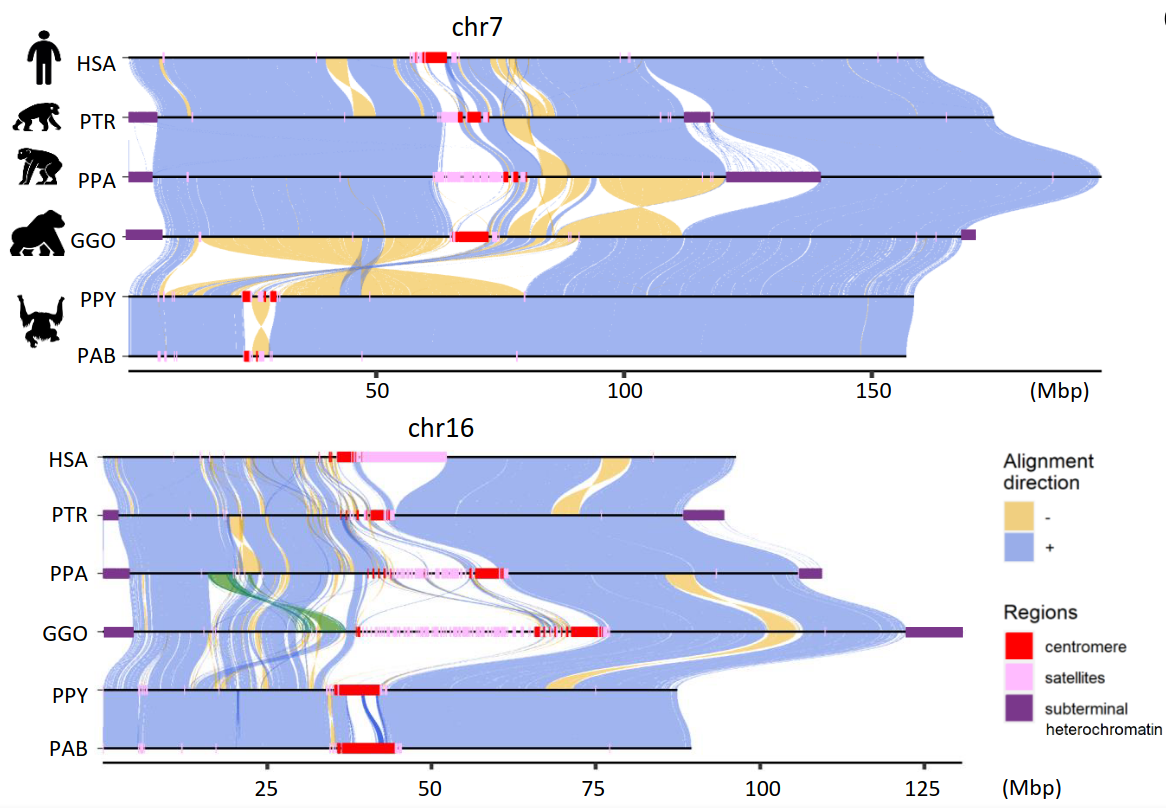
\includegraphics[width=\linewidth]{figures/background/genome_diff.png}
	\caption[Genomic difference in chromosome 7 and 16 of 5 primate species.]{A comparative ape alignment of human (HSA) chromosomes 7 and 16 with chimpanzee (PTR), bonobo (PPA), gorilla (GGO),Bornean and Sumatran orangutans (PPY and PAB). The image on the top shows most of the chromosome 7 is conserved except for large inversions happening between the species. The image below shows complex inversions in chromosome 16. Image taken from 'Complete sequencing of ape genomes'~\cite{ape_genomes}.}
	\label{fig:chromosome_diff}
\end{figure}

\begin{figure}[h!]\clearpage
	\centering
	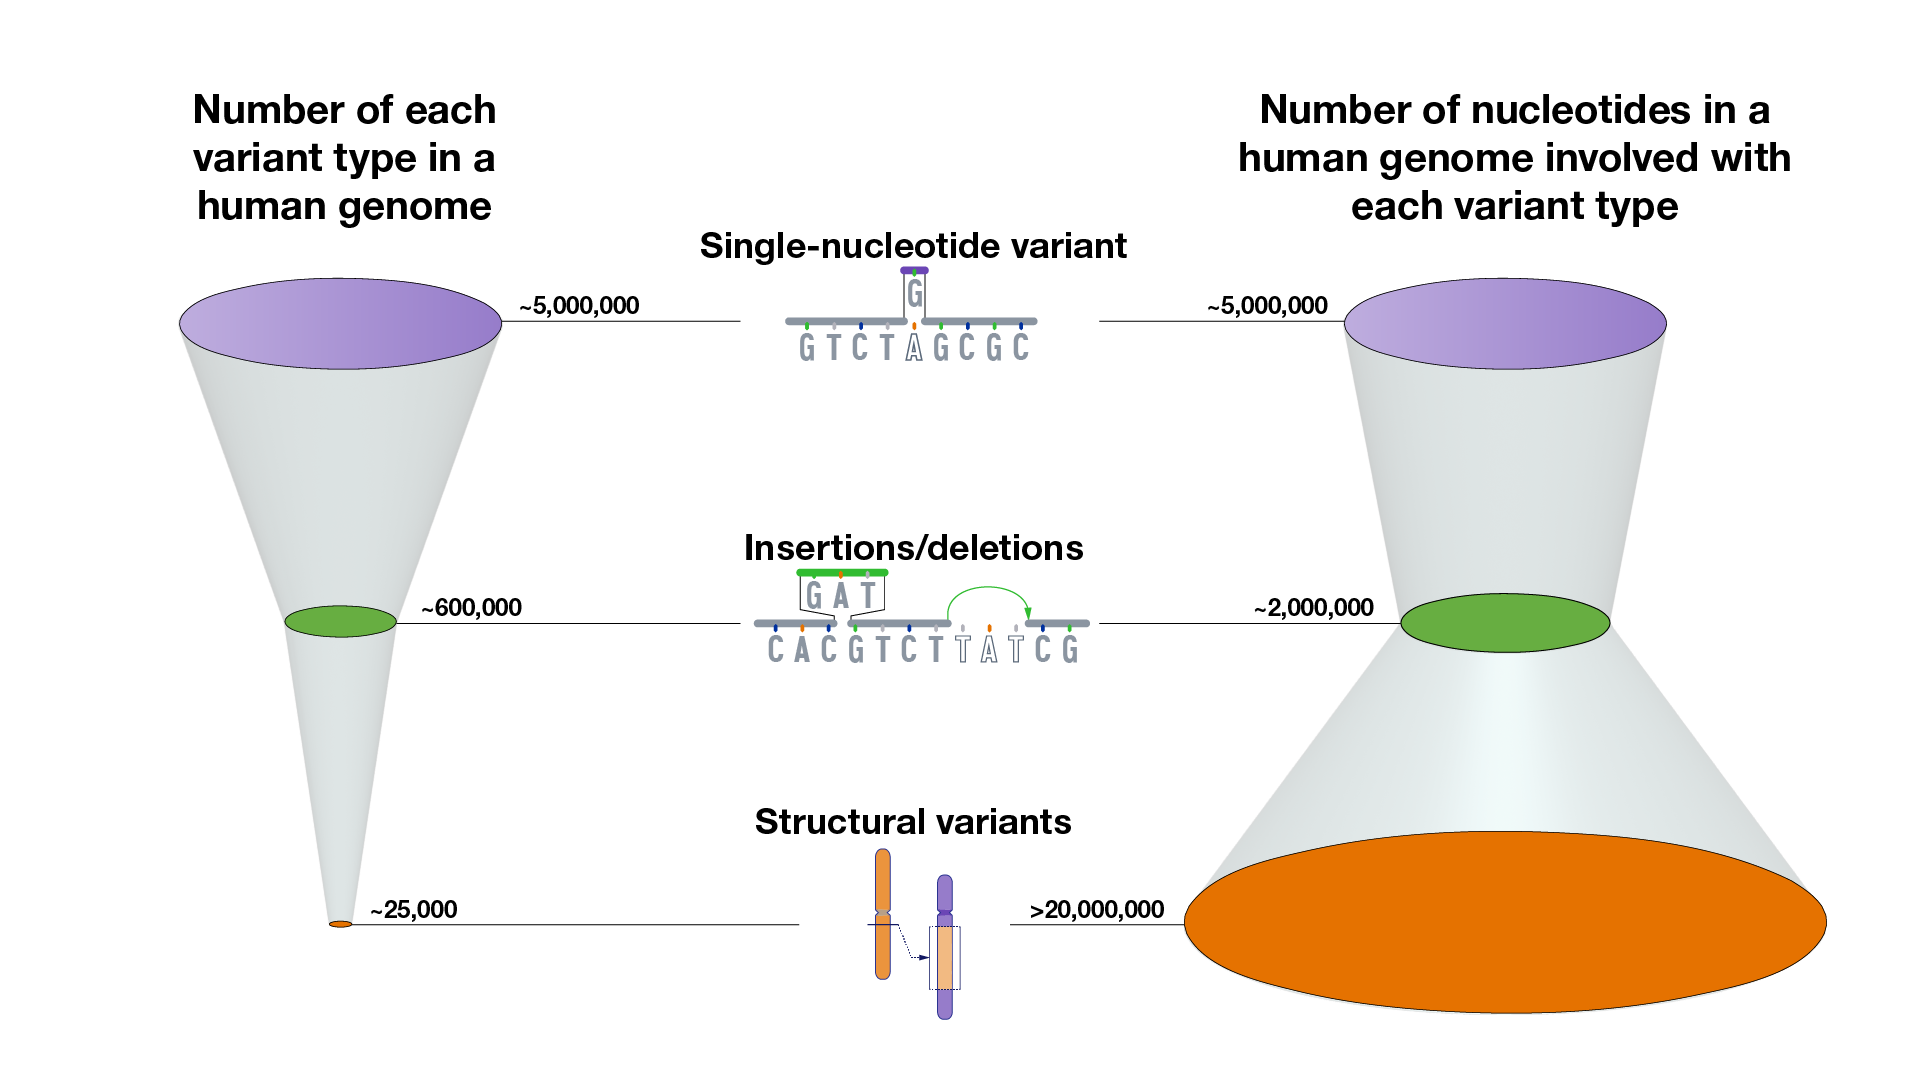
\includegraphics[width=.95\linewidth]{figures/background/genomic_spectrum.png}
	\caption[Spectrum of Human Genetic Variation.]{Spectrum of Human Genetic Variation. While SNPs are the most common variation event, their impact in the total amount of bases in a genome is ~4 times smaller than the one of Structural Variations, that are 200 times less frequent. This shows the great need to consider SVs in genomic analysis and not to stop at the SNP/indel level.\\}
	\label{fig:variation_spectrum}
\end{figure}

\section{Pangenomics, pangenomes and pangenome graphs}
\subsection{The premises for Pangenomics}
There are a number of factors that must be taken into consideration to understand one one side the need for a new paradigm and on the other side the conditions that lead to its development. Here I will briefly expose some of them before diving into pangenomics approaches and methods. 
\subsubsection{A single linear genome for all analyses}
Since the first complete genome sequences have been available in the late '90, all analysis based on sequencing data depended upon the use of a single linear reference genome, i.e. the best version of the genome available for any species. This reference sequence can or originate from the genome of a single organism or be a patch and consensus of multiple available genomes of the same species. It purpose is to use it infer information from newly, less refined, genomes that are being sequenced. We now know that this approach is suboptimal in a wide range of applications as a lot of genetic material of the species cannot be present in a single linear representation: this is valid for eukaryotes and even more for bacteria, that tend to be very diverse even in the same strain. The goal would therefore be to find a representation that provides more genetic material of a single species by intelligently combines the information from genome of multiple organisms and their differences.

\subsubsection{A quantity and quality revolution }
In the last few years we are witnessing a new revolution in sequencing. As the price of sequencing is lowering more than 2x per year, from 1\$/basepair to \$$10^-7$/basepair\cite{durbin_recomb}, new scientific discoveries and technological advances are leading to a remarkable increase of quality, in term of per-base error rate, and throughput of TGS. This means that in the next future we will dispose of a rich wealth of high quality sequencing information to produce hundreds or thousands of new first grade assemblies of large eukaryotic genomes. 

%This limitation at the beginning was not solvable due to the scarcity of high quality assembled genomes as the technologies of sequencing and computational tools were not mature enough.

For example, the history of complete human genome assemblies clearly exposes how much more high quality genomes it is now possible to generate. The Human Genome Project took 13 years to produce its result~\cite{humangenomeproject} and the absence of long reads with low error rate made it impossible to automatically resolve repetitive regions like telomeres and centromeres~\cite{human-pangenomics-era}, producing a reference only $92\%$ complete~\cite{t2t}. This problem was only solved in 2022 with a new, reference genome that did not have any gaps or unresolved regions, from the telomere to the other telomere of each chromosome~\cite{t2t}. Now, many consortia are producing increasingly more genomes to a level comparable to the one produced in 2022. For example, the HPRC, i.e. the Human Pangenome Reference Consortium, released 47 new human genomes (92 haplotypes) in 2021 and has recently released other 153 genomes to a total of 400 haplotypes of very high quality.

Finally, it is important to understand the quantity of biological information produced. As shown in table~\ref{tab:bp-increase}, the number of base pairs sequenced has more than doubled each year since 1995. As this is faster than the famous Moore's law on computing power, it is becoming evident that a new paradigm is needed to store and analyze such wealth of data. Public repositories, like Sequence Read Archive (SRA) and European Nucleotide Archive (ENA), are rapidly increasing the number of samples being sequenced and rendered publicly available to everyone, with tens of billions of millions of basepairs from genomic samples, as shown in figure~\ref{fig:SRA}. Other repositories of genomic data with associated medical metadata, like the UK biobank that comprises around 500 thousands individuals, are also emerging. These conditions are pushing the adoption of novel methods to process and analyze genomes.

\begin{table}[h!]
	\centering
	\begin{tabular}{c | c | c}
		year & genome(s) & base pairs \\
		1995 & Bacterium & $ 2*10^6$ \\
		2001 & Mammal & $ 3*10^9$ \\
		2013 & 2500 humans & $ 7.5*10^12$ \\
		2021 & ~1M genomes & $ 3*10^{15}$ \\
	\end{tabular}
	\caption[DNA data increase over the years.]{Base pairs had a $10^9$ increase in less than 30 years. As $10^9 ~~ 2^{30}$ (from $ \log_2(10^9) = 29.9$), the base pairs have more than doubled each year\cite{durbin_recomb}.}
	\label{tab:bp-increase}
\end{table}
\begin{figure}[h!]
	\centering
	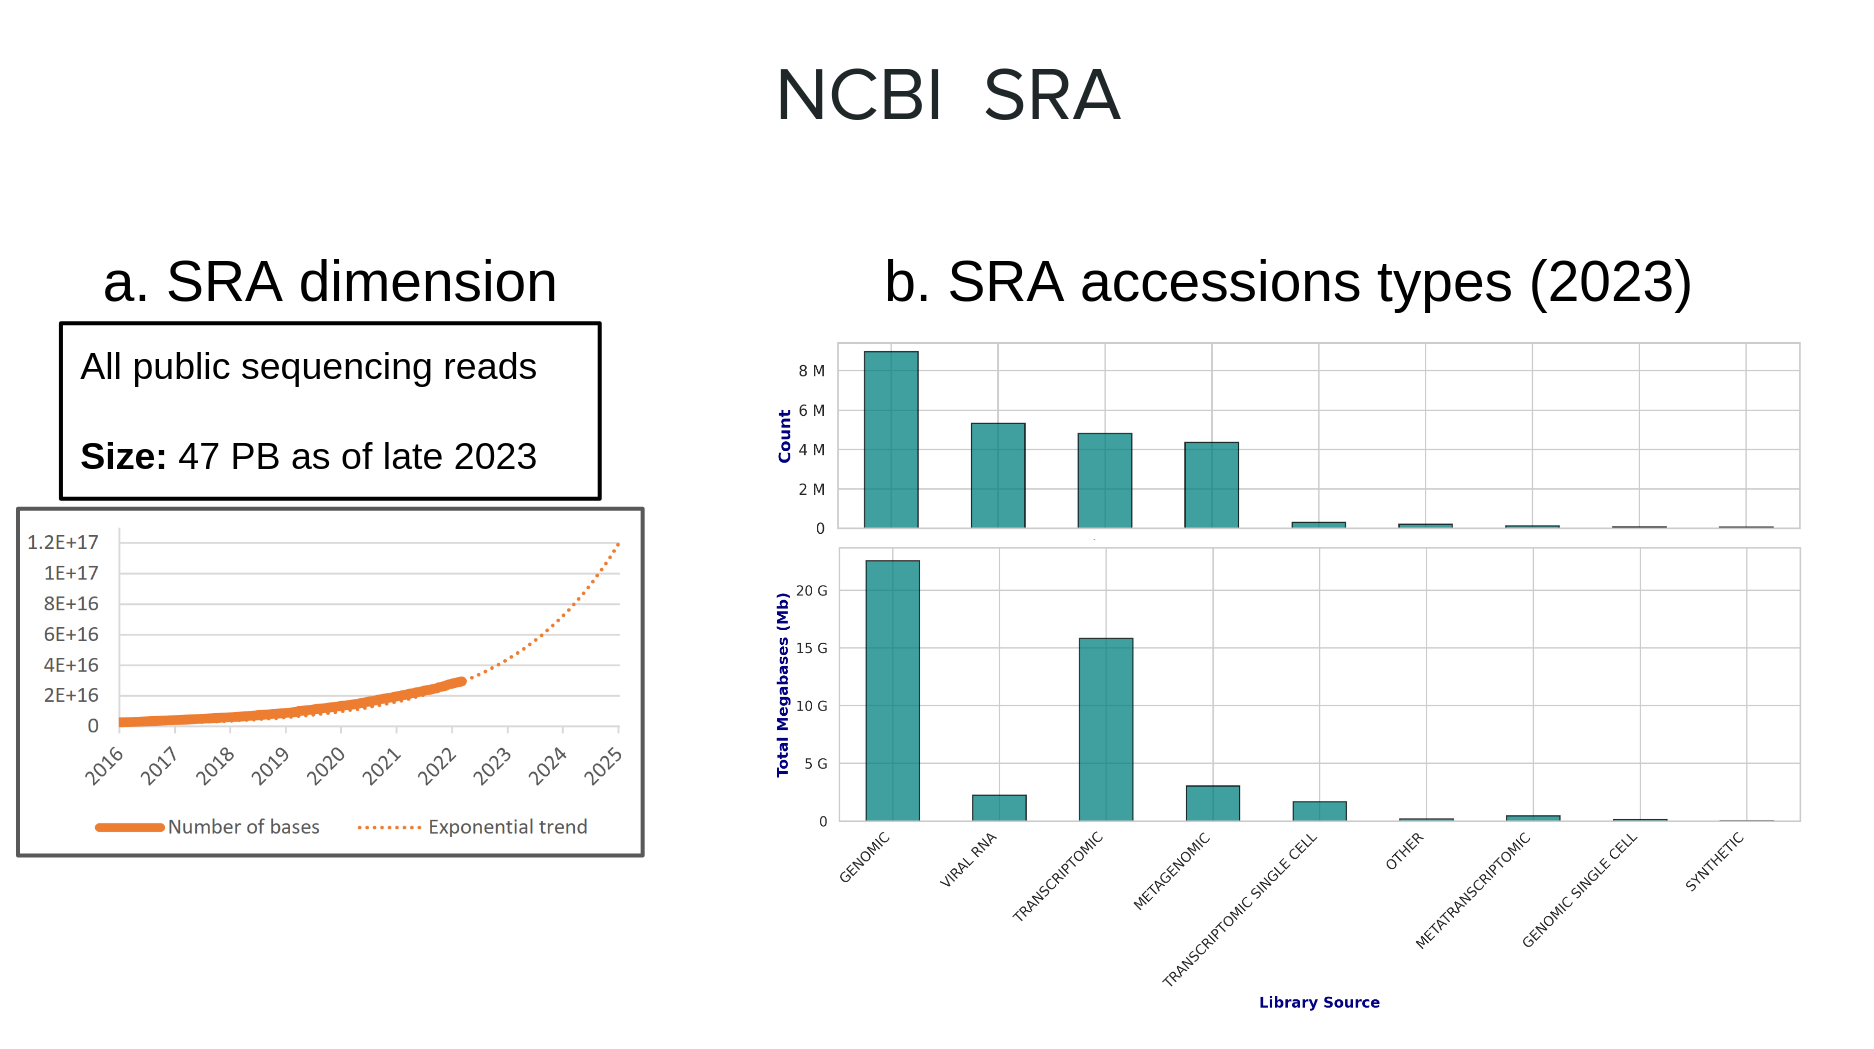
\includegraphics[width=\linewidth]{figures/background/sra.png}
	\caption[The Sequence Read Archive.]{a) The size in PetaBases (peta = $10^{15}$) of the SRA archive; b) The type of data in the SRA database shows the vast amount of genomic data available. Image made from Rayan Chikhi's slides.\\}
	\label{fig:SRA}
\end{figure}

\subsubsection{The need to better understand difference between genomes}
The ability to produce such good data is the main enabler of increasing efforts from the scientific community to propose new methods to analyze genomes: not anymore by comparing new genomes against a single good reference sequence but by comparing it in a comprehensive representation of the species. \\
Moreover, as new high quality sequences and assembled genomes are available, complex and/or highly repetitive regions can be now represented also for new genomes therefore enabling comparison between the ones of different genomes. This is very important as up until these improvement in sequencing and assemblies arrived, analyses were mostly blind to large, complex and/or repetitive structural variations. As we now know that these are the ones responsible for most of the difference between human genomes, new proposed approaches should provide new and better tools to understand, represent and analyze such variations.\\
Finally, as a single reference sequence cannot enclose all the possible structural variations of a population into a linear model, the need for a change in data structure for genomics arises.

%This novel way to overcome the limits of "linear genomic" and consider all the variation in a single species is called pangenomics. \\
%Various efforts are being made on producing reference pangenomes of yeasts, bacterias, plants and animals, including humans. In order to do so, new tools to construct and then analyse and use such representations are being developed. 
%It is important here to notice, as it will be stressed in the next sections and chapters, that construction is just the first step and that is very important to understand and work on which are the operations that can be succesfully performed by these representations. \\

\subsection{Pangenomics}
Pangenomics is therefore a rapidly evolving field in genomics that aims to capture and analyze the full genetic diversity within a species or a group of closely related species. It does not rely on a single, linear reference genome, but on comparing any genome with a group of other similar ones, as it seeks to represent all genetic variations and structural differences across collection of genomes. It leverages the availability of large collections of high quality assemblies of many species to overcome the observational bias of using a single haplotype as reference for a whole population. As shown in figure~\ref{fig:pangenomics_model}, the pangenome model aims at representing all variations among a group of complete genomes by describing the direct relationships between them, while in the linear model each genome is compared only to the reference: while in standard genomics genomes are compared between each other via indirect difference to the linear reference, in pangenomics the comparison is direct. When a new genome is added to a collection, in genomics it compares just to the reference while in pangenomics it does with all the genomes present in the model.
\begin{figure}[h!]
	\centering
	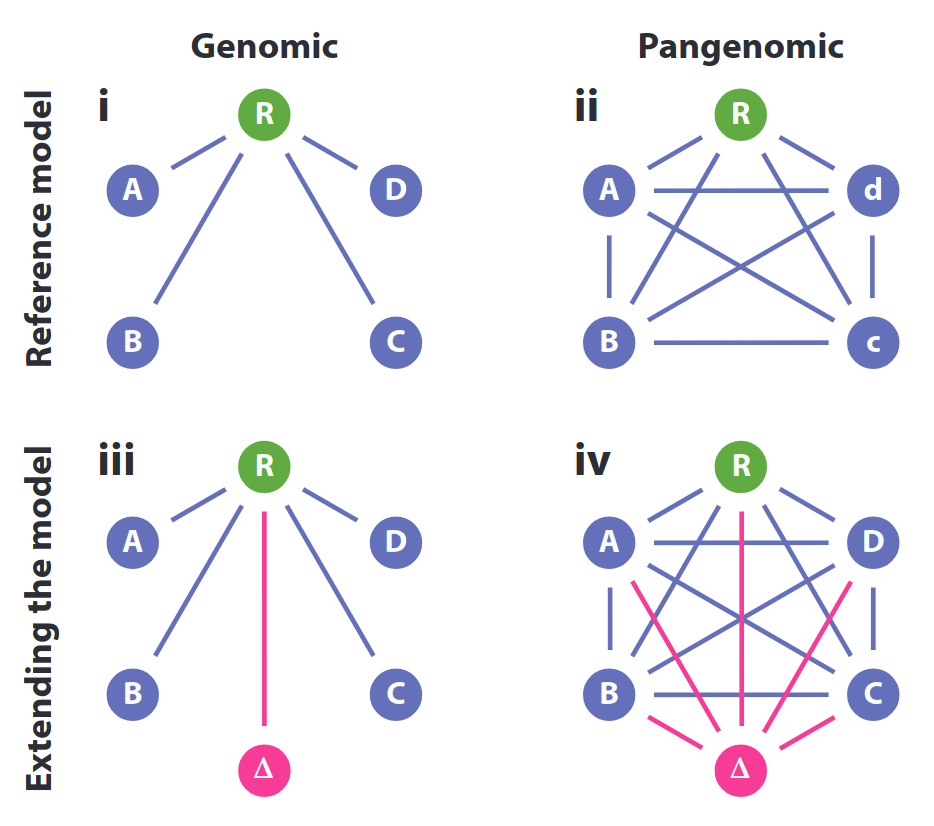
\includegraphics[width=.75\linewidth]{figures/background/pangenome_model.png}
	\caption[The Pangenome model.]{The genomic vs pangenomic model i) In the genomic model each genome is compared only to the reference sequence. Any comparison between a pair of genomes is done indirectly via their difference with the reference. ii) In the pangenomics, variations are described in a relative way for any genome. Any pair of genomes can be compared directly. iii) In the genomic model, to add a new genome in the collection it has to be compared to the reference. iv) In pangenomics, each new genomes added to the model is automatically compared to all the ones in the collection. Figure from~\cite{eizenga}\\}
	\label{fig:pangenomics_model}
\end{figure}
It was first conceptualized for bacterial genomes, and at gene level, without considering non coding regions. This was mostly due to the fact that bacteria share genes between each other, generating high diversity in the gene repertoire between organisms of the same species or strain.
The first proposed pangenome model had a subdivision between a core genome, made by genes present in all individuals of a species, and a dispensable or accessory genome, with genes present in some, but not all, individuals.\\
This definition would then extend to a more general model that would consider variations at the nucleotide level to contain all variations in a set of genomes.\\
\subsubsection{Pangenomes}
A pangenome can be therefore be considered any collection of genomic sequences to be analyzed jointly or to be used as reference. This definition provides two important concepts for the rest of the studies provided in this manuscript: 
\begin{itemize}
	\item[\textbf{Model}] the pangenome is not a well-defined structure or model but can be from a simple collection of sequences to complex data structures. This means that different approaches are developed and used depending on the application of interest;
	\item[\textbf{scope}] a pangenome can be either used as:
	\begin{itemize}
		\item a new reference for a specific species to be used for analyses in a similar way as linear genome. This means that a large consortium would be producing a representation that is accepted as new standard. For the Human genome this is done by the HPRC consortium as the T2T consortium produced the best-quality linear reference genome~\cite{t2t}.
		\item a different model that can be used to study a set of genomes, without needing \emph{a priori} to use a reference. This model can find applications in population variation studies. 
	\end{itemize} 
\end{itemize}
Pangenomes can be an unaligned set of sequences. This is the most basic case, with no processing of the data but that conserve the full information from the assembly without introducing any bias or error. In this sense, a group of complete genomes of a family, species or genera can be considered a basic form of pangenome. They can be used together to infer direct relationships between each other, via alignment. For example, as the T2T consortium has fully resolved the centromeres of 2 human genomes, when considered together, it is possible to detect small-scale and large-scale centromere variations, something that was never possible before~\cite{centromeres_eichler}. By having high quality assemblies of various apes, it is possible to reconstruct complex and large variations and rearrangements in chromosomes between them and the human genome that could not be detected before~\cite{apes_genomes}.\\
A multiple sequence alignment (MSA) of haplotype-resolved complete genomes can be considered a pangenome. This data structure originated from complex and costly alignment operations is the basis of many computational approaches, also in pangenomics, like the founder graphs. These models are limited in scope as it is impractical as it does not work well when genomes are too large, have complex variations or are very divergent.\\
Pangenomes can be also represented as sets of \kmers. This approach has several advantages: it scales very well to large collections of genomes, accepts as input from raw reads to complete assemblies and is unbiased. The drawbacks mostly consist on the right choice of the \kmer length and the 

\subsubsection{Pangenome Graphs}
Graphs are a natural way of directly representing information between a group of object that share some properties: they provide a human interface to a set of relationships. \\
A graph is a mathematical structure used to represent associations between abstract entities. It consists of two main components:
\begin{itemize}[leftmargin=1.8cm]
	\item[\smash{\stackunder{\textbf{Nodes}}{\textbf{(vertices)}}}] are the entities of the graph that possess some properties (like a value or label);
	\item[\textbf{Edges}] are the connections between the nodes that represent the interactions between the nodes (shared property or difference).
\end{itemize}
Graphs are widely used in a lot of applications, mainly to describe and interpret complex structures in social, transportation or computer networks.\\
Graphical models are largely adopted to represent pangenomes. They differ in the property associated to the vertices and therefore in the information provided by the edges.
\begin{itemize}[leftmargin=1.8cm]
	\item[{\smash{\stackunder{\textbf{De Bruijn}}{\textbf{graph}}}}] have nodes with labels representing \kmers and overlap relationship between \kmers is expressed using edges; \kmers and their reverse complement are represented by the same node, so the graph is bidirected, with edges connecting a strand of a node label to another strand of a node label.
	\item[{\smash{\stackunder{\textbf{Directed genome}}{\textbf{graph}}}}] have nodes labels representing a sequence and edges signal adjacency of two sequences in at least one genome. A sequence and its reverse complement are assigned to two different nodes, as the only information represented by the graph is the contiguity of pairs of sequences.
	\item[{\smash{\stackunder{\textbf{Bidirected genome}}{\textbf{graph}}}}] have nodes with a label and two sides, i.e. the start and the end of the label. Edges connect one side of a label to the side of another, to provide the starting point of the sequence spelled. If a node is traversed from left to right, it is the forward strand of the sequence, if done right to left, it is the reverse strand of the DNA~\cite{odgi}.
\end{itemize}
\begin{figure}[h!]
	\centering
	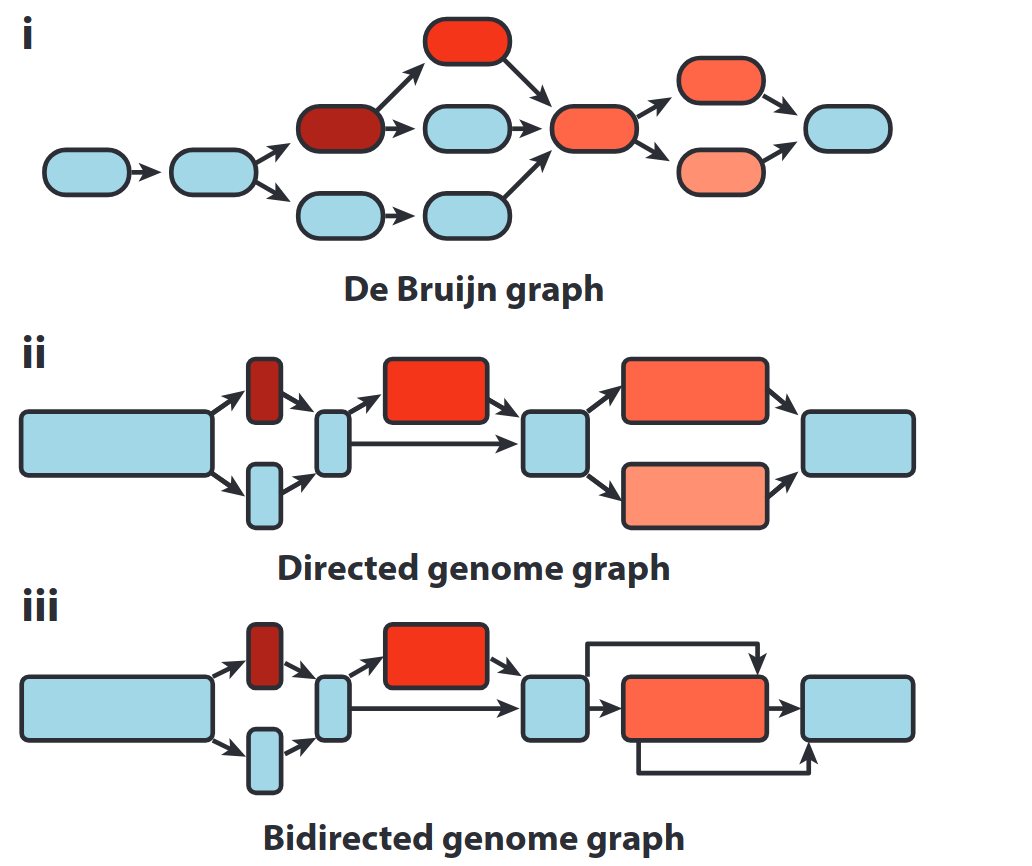
\includegraphics[width=.75\linewidth]{figures/background/graph_types.png}
	\caption[Graph pangenome models.]{The three main kind of graphs used to represent pangenomes. Figure from~\cite{eizenga}}
	\label{fig:graph_types.png}
\end{figure}
The choice of a particular model relies mostly on which is the envisioned application: there is no one-fits-all solution because of trade-offs between optimal desiderata. A model that enables useful visualization can be not suited for large collections of genomes, other that allow the addition of new genomes without recomputing everything from scratch, also called dynamical-updates, are not the best for efficient compression and storage and so on.\\
Genomic variations in graphs consist of bubbles representing alternative paths between a source node and an end node. Different variations produce different kind of bubbles and different models produce bubbles with different patterns. Two examples for \dbg and genome graph can be seen in figure\ref{fig:vg_example,fig:dbg_ex}\\
Below I present the two main models actually used for pangenome graphs construction: Variation graphs and De Bruijn graphs.

\subsection{Variation Graphs}
Variation graph are an enhancement of bidirected genome graphs with paths. Paths correspond to walks in the graph that visit nodes in an assigned orientation to reproduce sequences provided as input, as shown in figure~\ref{fig:vg_example}. It therefore consists of a bidirected genome graph constructed from the sequences in the input genomes plus a list of paths that spell such sequences inside the graph.
\begin{figure}[h!]
	\centering
	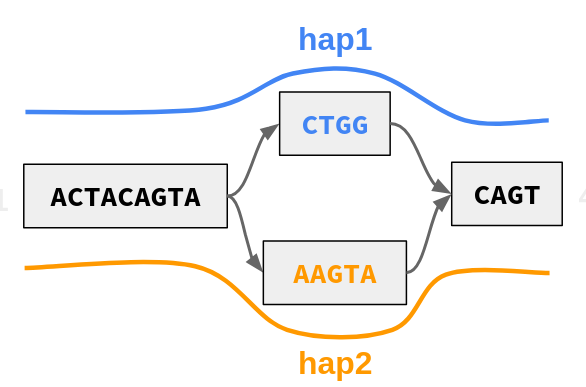
\includegraphics[width=.65\linewidth]{figures/background/vg.png}
	\caption[The Variation Graph model.]{An example of variation graph, in which haplotype1 spells the sequence \emph{ACTACAGTACTGGCAGT}, while haplotype 2 spells the sequence \emph{ACTACAGTAAAGTACAGT}~\cite{garrison_pangenome}.}
	\label{fig:vg_example}
\end{figure}
This data structure has been first proposed to represent textual variations. As shown in figure~\ref{fig:campagna_romana}, the variation graphs represent the conservation and variation in a system: it is therefore a very good model to represent the direct relationships between a group of genomes.
\begin{figure}[h!]
	\centering
	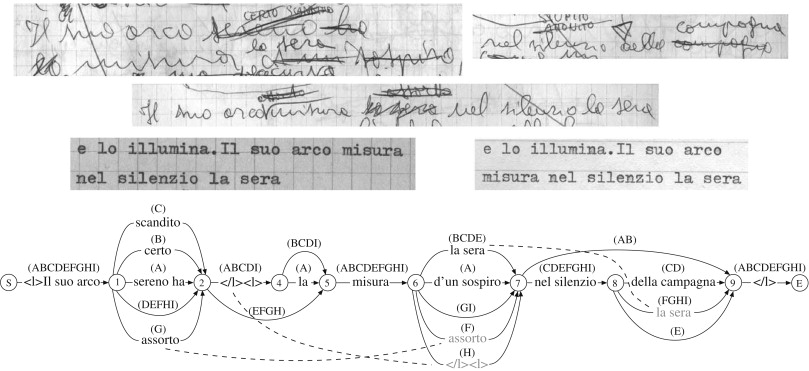
\includegraphics[width=.95\linewidth]{figures/background/variant_graph.jpg}
	\caption[The Variation Graph origin.]{Instead of having to preform all the pairwise comparisons of the nine version of Valerio Magrelli's "Campagna Romana" poem from 1981, the variation graph structure describes the differences between them. It also removes the high redundancy in the versions of the poem~\cite{variant_graph,garrison_pangenome}.}
	\label{fig:campagna_romana}
\end{figure}
Variation graphs of genomes can now be constructed thanks to the advent of TGS and complete high quality assembly pipelines. As already discussed, genomes are full of repeats, making assembly is hard, especially if the only information available is reads shorter than the repeat sequences, as with NGS.\\
Variation graphs can be generated in a direct, all-v-all unbiased way or in a iterative, reference driven manner.
The pros of using a variation graph are:
\begin{itemize}
	\item variation is intuitive when visualizing the graph
\end{itemize}



\subsection{De Bruijn Graphs}
As variation graphs, \dbgs are not born with pangenomics. They are a well-known data structure that found great application in genome assembly, especially with NGS.
A \dbg is a data structure that represent a collection of input sequences as a set of \kmers. It therefore reduces the redundancy in the data by storing only once each unique \kmer seen in the input. The graph has as node labels the \kmers and directed edges between nodes indicate \emph{k-1} overlap between the two \kmers. \dbgs are also bidirected, as each \kmer encodes also its reverse complement: the one present in the label of the node is usually the canonical one. Bidirected edges encode the strandness of the \kmer of the starting node as well as the one of the ending node. 
\begin{figure}[h!]
	\centering
	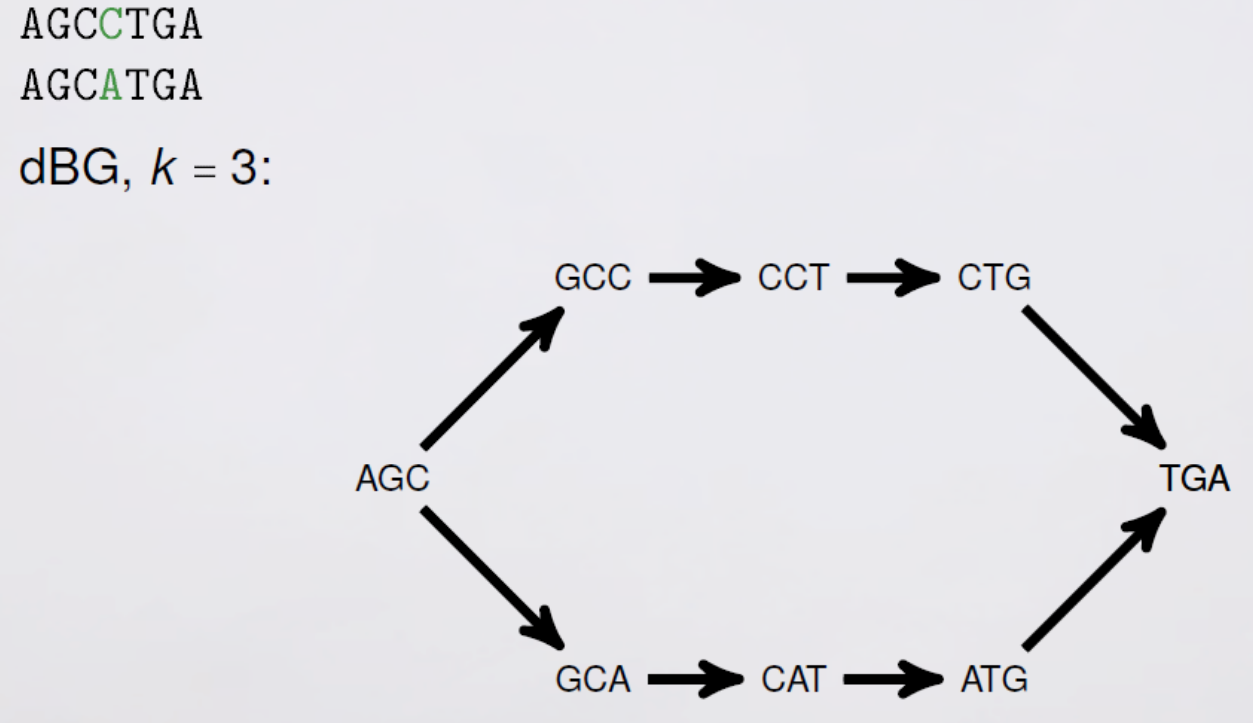
\includegraphics[width=.95\linewidth]{figures/background/dbg.png}
	\caption[Example of \dbg.]{Example of \dbg for $k=3$ with a bubble representing a SNP.}
	\label{fig:dbg_ex}
\end{figure}
The choice of $k$ depends on multiple factors and in fact is a trade-off between: 
\begin{itemize}
	\item[Specificity] The larger the $k$, the sparser is the set of \kmers of the \dbg in the space. While smaller $k$ (21-31) is more general and fits most solutions, larger $k$ (61-100) provides more specificity. This is because 2 or more genomes are have greater probability of sharing small subsequences than large ones.
	\item[Variation resolution] While variation is always encoded in a \dbg, larger $k$ values produce a sparser graph, in which there are less nodes with label \kmers that are repeated multiple times in the genome. This means that once visualizing a specific region of the graph, it is possible to detect local variations and not be confounded by other nodes and edges coming from other part of the genomes that share \kmers present in the region.
	\item[Space] As shown in in table~\ref{tab-kmers}, larger value of $k$ produces more redundancy and a greater number of basepairs with the same input sequences. If the collection to study is large, smaller $k$ can provide beneficial features for disk storage or computational resources needed when using it.
\end{itemize}
\subsubsection{Colored and Compacted De Bruijn Graphs}
In order to produce a more compact and informative representation, in pangenomics it is used a particular version of the \dbg that 
\begin{itemize}
	\item compacts simple paths (no branching or bubbles), i.e. if there is a chain of at least two nodes that have just one entering edge and just one outgoing edge, the nodes gets compacted into a single one and the label becomes the extension of the first \kmer with the last nucleotide of the labels of the subsequent nodes. Such labels are no longer of length $k$ and thus are not \kmers: they are called unitigs and provide a more succinct representation of the \kmers in the \dbg~\ref{fig:ccdbg}.
	\item stores for each \kmer (also inside unitigs), the genome in which it has been seen: this information is called color. The color of each \kmer in the \ccdbg is stored in a very compressed way in order to reduce space. Colors allow useful analysis by not only using the presence or absence of a \kmer in a \dbg but also in which genomes it was observed.
\end{itemize}
While \kmer compaction into unitigs can be done at a second moment starting from a \dbg, novel methods tend to compute unitigs directly, without passing for the \dbg construction.\\
Colors can be a confusing term as it is used for two different cases: they can represent directly the dataset of origin or they can represent any combination of dataset of origin that is seen associated to a \kmer (also called color sets)~\cite{marchet_kmersets}. The color sets is the most used model as, instead of remembering for each \kmer which are the datasets in which it is contained, it assign an integer to any combination of dataset seen and then associate it to the \kmers, in order to save space, as shown in figure~\ref{fig:ccdbg}. 
\begin{figure}[h!]
	\centering
	\begin{subfigure}[b]{0.95\textwidth}
		\centering
		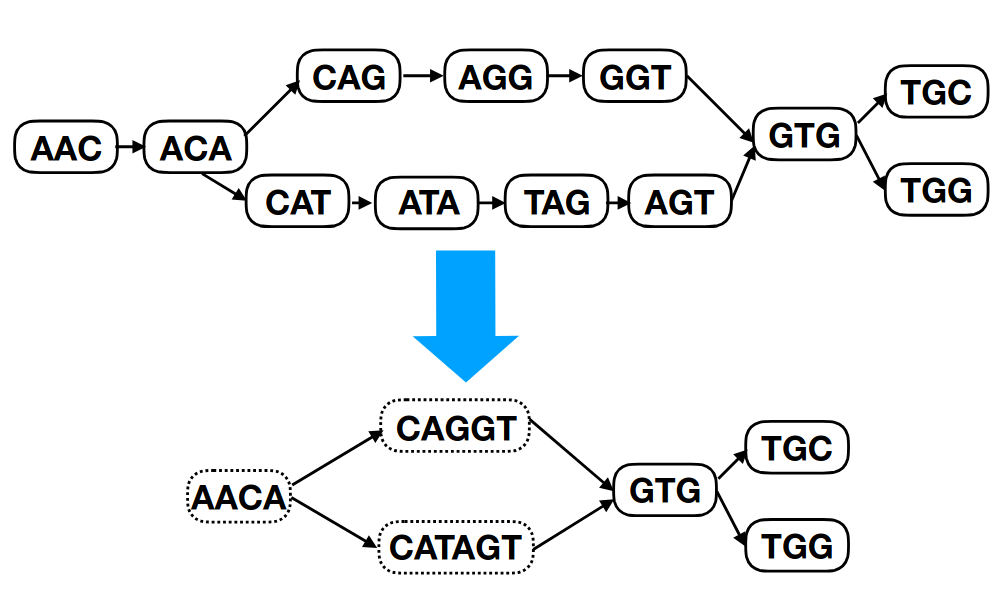
\includegraphics[width=.75\linewidth]{figures/background/compacting.png}
		\caption[Compacting a \dbg.]{Compacting a \dbg from the two sequences \texttt{AACAGGTGC} and \texttt{AACATAGTGG} into a \cdbg reduces paths of nodes with in-degree and out-degree of 1 into a single node. Figure from~\cite{embedding_dbg}}
	\end{subfigure}%
	\\
	\begin{subfigure}[b]{0.95\textwidth}
		\centering
		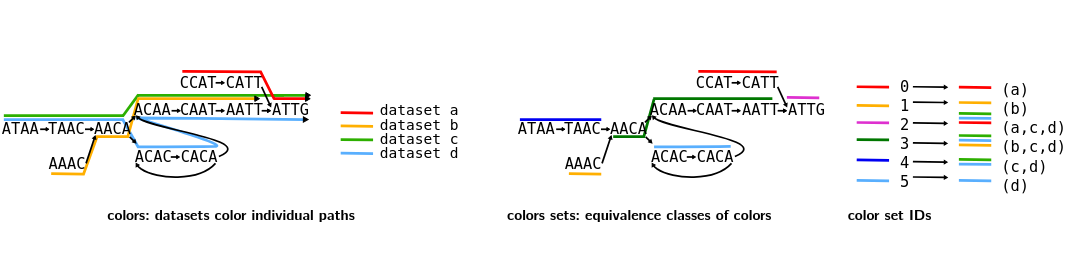
\includegraphics[width=0.95\textwidth]{figures/background/colors_dbg.png}
		\caption[The colors in a \ccdbg.]{The two kind of colors that can be used on \ccdbg: colors and color sets.} 
	\end{subfigure}%
	\caption[Compaction and colors in a \ccdbg.]{Compaction and colors: the two main characteristic of a \ccdbg compared to a \dbg. Figure from~\cite{marchet_kmersets}}
	\label{fig:ccdbg}
\end{figure}

\section{Outline}
In the work presented below, we investigate the graphical pangenome representation on the features presented in the sections above. We focused mainly on the construction of such models, their underlying data structures and the downstream application they enable.\\
The contributions presented in this paper are the following:
\begin{enumerate}
	\item \textbf{An analysis of pangenome construction methods and their applications}. Even if the variation graph model has been devised around 15 years ago, its application for pangenomics is very recent. \dbgs are instead a known model that has been extensively used for genome assembly and their application to pangenomics is relatively straightforward. We used all the state-of-the-art tools to produce pangenome graph based on these two representations using a large collection of complete human genomes and tested computational resources, variation representation and applications.
	\item  \textbf{A novel construction of pathogenic yeast strains to discover chromosomal translocations.} Pangenome graphs can be used to investigate complex structural variations in genomes. In this case we sequenced, assembled and analyzed a group of 11 samples. We modified a variation graph construction pipeline to detect cross-chromosome events and discussed differences in the final representation.
	\item \textbf{A unitig matrix construction pipeline for presence/absence or counts.} We proposed a small pipeline, based on already published tools and a novel method, \texttt{kmattool}, a pipeline to build unitig matrices with abundances from a set of genomes via \kmer matrix and to directly generate a presence absence unitig matrix using \ccdbgs. 
	\item  \textbf{A novel superkmers enumeration and sorting method based on a special representation.} We propose a novel way to encode and store superkmers that preserves locality for the ones sharing the same minimizer to improve sequence queries. We also propose a tool to enumerate and sort superkmers from a set of sequences using this model.
\end{enumerate}
The next chapters present this work and discuss the possible directions for future work based on it.

\printbibliography